\documentclass[twoside]{book}

% Packages required by doxygen
\usepackage{calc}
\usepackage{doxygen}
\usepackage{graphicx}
\usepackage[utf8]{inputenc}
\usepackage{makeidx}
\usepackage{multicol}
\usepackage{multirow}
\usepackage{textcomp}
\usepackage[table]{xcolor}

% Font selection
\usepackage[T1]{fontenc}
\usepackage{mathptmx}
\usepackage[scaled=.90]{helvet}
\usepackage{courier}
\usepackage{amssymb}
\usepackage{sectsty}
\renewcommand{\familydefault}{\sfdefault}
\allsectionsfont{%
  \fontseries{bc}\selectfont%
  \color{darkgray}%
}
\renewcommand{\DoxyLabelFont}{%
  \fontseries{bc}\selectfont%
  \color{darkgray}%
}

% Page & text layout
\usepackage{geometry}
\geometry{%
  a4paper,%
  top=2.5cm,%
  bottom=2.5cm,%
  left=2.5cm,%
  right=2.5cm%
}
\tolerance=750
\hfuzz=15pt
\hbadness=750
\setlength{\emergencystretch}{15pt}
\setlength{\parindent}{0cm}
\setlength{\parskip}{0.2cm}
\makeatletter
\renewcommand{\paragraph}{%
  \@startsection{paragraph}{4}{0ex}{-1.0ex}{1.0ex}{%
    \normalfont\normalsize\bfseries\SS@parafont%
  }%
}
\renewcommand{\subparagraph}{%
  \@startsection{subparagraph}{5}{0ex}{-1.0ex}{1.0ex}{%
    \normalfont\normalsize\bfseries\SS@subparafont%
  }%
}
\makeatother

% Headers & footers
\usepackage{fancyhdr}
\pagestyle{fancyplain}
\fancyhead[LE]{\fancyplain{}{\bfseries\thepage}}
\fancyhead[CE]{\fancyplain{}{}}
\fancyhead[RE]{\fancyplain{}{\bfseries\leftmark}}
\fancyhead[LO]{\fancyplain{}{\bfseries\rightmark}}
\fancyhead[CO]{\fancyplain{}{}}
\fancyhead[RO]{\fancyplain{}{\bfseries\thepage}}
\fancyfoot[LE]{\fancyplain{}{}}
\fancyfoot[CE]{\fancyplain{}{}}
\fancyfoot[RE]{\fancyplain{}{\bfseries\scriptsize Generated on Tue Nov 14 2017 15\-:01\-:38 for Face Verification for an Acess Control System by Doxygen }}
\fancyfoot[LO]{\fancyplain{}{\bfseries\scriptsize Generated on Tue Nov 14 2017 15\-:01\-:38 for Face Verification for an Acess Control System by Doxygen }}
\fancyfoot[CO]{\fancyplain{}{}}
\fancyfoot[RO]{\fancyplain{}{}}
\renewcommand{\footrulewidth}{0.4pt}
\renewcommand{\chaptermark}[1]{%
  \markboth{#1}{}%
}
\renewcommand{\sectionmark}[1]{%
  \markright{\thesection\ #1}%
}

% Indices & bibliography
\usepackage{natbib}
\usepackage[titles]{tocloft}
\setcounter{tocdepth}{3}
\setcounter{secnumdepth}{5}
\makeindex

% Hyperlinks (required, but should be loaded last)
\usepackage{ifpdf}
\ifpdf
  \usepackage[pdftex,pagebackref=true]{hyperref}
\else
  \usepackage[ps2pdf,pagebackref=true]{hyperref}
\fi
\hypersetup{%
  colorlinks=true,%
  linkcolor=blue,%
  citecolor=blue,%
  unicode%
}

% Custom commands
\newcommand{\clearemptydoublepage}{%
  \newpage{\pagestyle{empty}\cleardoublepage}%
}


%===== C O N T E N T S =====

\begin{document}

% Titlepage & ToC
\hypersetup{pageanchor=false}
\pagenumbering{roman}
\begin{titlepage}
\vspace*{7cm}
\begin{center}%
{\Large Face Verification for an Acess Control System }\\
\vspace*{1cm}
{\large Generated by Doxygen 1.8.6}\\
\vspace*{0.5cm}
{\small Tue Nov 14 2017 15:01:38}\\
\end{center}
\end{titlepage}
\clearemptydoublepage
\tableofcontents
\clearemptydoublepage
\pagenumbering{arabic}
\hypersetup{pageanchor=true}

%--- Begin generated contents ---
\chapter{Main Page}
\label{index}\hypertarget{index}{} Project developed by Daniel Lopes, Ricardo Ribeiro and António Neves. 
\chapter{Namespace Index}
\section{Namespace List}
Here is a list of all documented namespaces with brief descriptions\-:\begin{DoxyCompactList}
\item\contentsline{section}{\hyperlink{namespaceauxiliary}{auxiliary} }{\pageref{namespaceauxiliary}}{}
\item\contentsline{section}{\hyperlink{namespacefacetracker}{facetracker} }{\pageref{namespacefacetracker}}{}
\item\contentsline{section}{\hyperlink{namespaceimg__screen}{img\-\_\-screen} }{\pageref{namespaceimg__screen}}{}
\item\contentsline{section}{\hyperlink{namespaceimg__screen__entry}{img\-\_\-screen\-\_\-entry} }{\pageref{namespaceimg__screen__entry}}{}
\item\contentsline{section}{\hyperlink{namespaceNFC__Arduino}{N\-F\-C\-\_\-\-Arduino} }{\pageref{namespaceNFC__Arduino}}{}
\item\contentsline{section}{\hyperlink{namespaceRecognitionFactory}{Recognition\-Factory} }{\pageref{namespaceRecognitionFactory}}{}
\item\contentsline{section}{\hyperlink{namespaceregister__facetracker}{register\-\_\-facetracker} }{\pageref{namespaceregister__facetracker}}{}
\item\contentsline{section}{\hyperlink{namespaceregister__server}{register\-\_\-server} }{\pageref{namespaceregister__server}}{}
\item\contentsline{section}{\hyperlink{namespacesend__socket}{send\-\_\-socket} }{\pageref{namespacesend__socket}}{}
\item\contentsline{section}{\hyperlink{namespaceverification__server}{verification\-\_\-server} }{\pageref{namespaceverification__server}}{}
\end{DoxyCompactList}

\chapter{Hierarchical Index}
\section{Class Hierarchy}
This inheritance list is sorted roughly, but not completely, alphabetically\-:\begin{DoxyCompactList}
\item \contentsline{section}{Calibration}{\pageref{classCalibration}}{}
\item \contentsline{section}{Camera}{\pageref{classCamera}}{}
\item object\begin{DoxyCompactList}
\item \contentsline{section}{Recognition\-Factory.\-Recognition\-Algorithm}{\pageref{classRecognitionFactory_1_1RecognitionAlgorithm}}{}
\begin{DoxyCompactList}
\item \contentsline{section}{Recognition\-Factory.\-d\-Lib}{\pageref{classRecognitionFactory_1_1dLib}}{}
\item \contentsline{section}{Recognition\-Factory.\-Open\-Face}{\pageref{classRecognitionFactory_1_1OpenFace}}{}
\end{DoxyCompactList}
\end{DoxyCompactList}
\end{DoxyCompactList}

\chapter{Class Index}
\section{Class List}
Here are the classes, structs, unions and interfaces with brief descriptions\+:\begin{DoxyCompactList}
\item\contentsline{section}{\hyperlink{classRecognitionFactory_1_1DeepFace}{Recognition\+Factory.\+Deep\+Face} }{\pageref{classRecognitionFactory_1_1DeepFace}}{}
\item\contentsline{section}{\hyperlink{classDetectionFactory_1_1DetectionAlgorithm}{Detection\+Factory.\+Detection\+Algorithm} }{\pageref{classDetectionFactory_1_1DetectionAlgorithm}}{}
\item\contentsline{section}{\hyperlink{classRecognitionFactory_1_1dLib}{Recognition\+Factory.\+d\+Lib} }{\pageref{classRecognitionFactory_1_1dLib}}{}
\item\contentsline{section}{\hyperlink{classDetectionFactory_1_1dLib}{Detection\+Factory.\+d\+Lib} }{\pageref{classDetectionFactory_1_1dLib}}{}
\item\contentsline{section}{\hyperlink{classfacenet_1_1ImageClass}{facenet.\+Image\+Class} }{\pageref{classfacenet_1_1ImageClass}}{}
\item\contentsline{section}{\hyperlink{classDetectionFactory_1_1MTCNN}{Detection\+Factory.\+M\+T\+C\+NN} }{\pageref{classDetectionFactory_1_1MTCNN}}{}
\item\contentsline{section}{\hyperlink{classdetect__face_1_1Network}{detect\+\_\+face.\+Network} }{\pageref{classdetect__face_1_1Network}}{}
\item\contentsline{section}{\hyperlink{classdetect__face_1_1ONet}{detect\+\_\+face.\+O\+Net} }{\pageref{classdetect__face_1_1ONet}}{}
\item\contentsline{section}{\hyperlink{classRecognitionFactory_1_1OpenFace}{Recognition\+Factory.\+Open\+Face} }{\pageref{classRecognitionFactory_1_1OpenFace}}{}
\item\contentsline{section}{\hyperlink{classdetect__face_1_1PNet}{detect\+\_\+face.\+P\+Net} }{\pageref{classdetect__face_1_1PNet}}{}
\item\contentsline{section}{\hyperlink{classRecognitionFactory_1_1RecognitionAlgorithm}{Recognition\+Factory.\+Recognition\+Algorithm} }{\pageref{classRecognitionFactory_1_1RecognitionAlgorithm}}{}
\item\contentsline{section}{\hyperlink{classdetect__face_1_1RNet}{detect\+\_\+face.\+R\+Net} }{\pageref{classdetect__face_1_1RNet}}{}
\end{DoxyCompactList}

\chapter{Namespace Documentation}
\hypertarget{namespaceauxiliary}{\section{auxiliary Namespace Reference}
\label{namespaceauxiliary}\index{auxiliary@{auxiliary}}
}
\subsection*{Functions}
\begin{DoxyCompactItemize}
\item 
def \hyperlink{namespaceauxiliary_af0a4ce60dc31d830c176285588b149ef}{yaw\-\_\-movement}
\begin{DoxyCompactList}\small\item\em It will select if the face image is suitable or not to be sent to the verification system according to the yaw movement of the head towards the camera. \end{DoxyCompactList}\item 
def \hyperlink{namespaceauxiliary_ae22d1d7827aa2906a00e6fac8fc9c2ef}{blink\-\_\-eyes}
\begin{DoxyCompactList}\small\item\em It will select if the face image is suitable or not to be sent to the verification system according to the eyes of the person. \end{DoxyCompactList}\item 
\hypertarget{namespaceauxiliary_a5bb7e810a9ce859f0f4ce787bb8f74cf}{def \hyperlink{namespaceauxiliary_a5bb7e810a9ce859f0f4ce787bb8f74cf}{save\-\_\-descriptors\-\_\-array}}\label{namespaceauxiliary_a5bb7e810a9ce859f0f4ce787bb8f74cf}

\begin{DoxyCompactList}\small\item\em In construction phase. \end{DoxyCompactList}\item 
\hypertarget{namespaceauxiliary_a711c0b5a01a24683b3ba2c6eca1b96e1}{def \hyperlink{namespaceauxiliary_a711c0b5a01a24683b3ba2c6eca1b96e1}{send\-\_\-descriptors\-\_\-socket}}\label{namespaceauxiliary_a711c0b5a01a24683b3ba2c6eca1b96e1}

\begin{DoxyCompactList}\small\item\em In construction phase. \end{DoxyCompactList}\item 
\hypertarget{namespaceauxiliary_a681eebd7d4f0632ca527d000d79fbc5c}{def \hyperlink{namespaceauxiliary_a681eebd7d4f0632ca527d000d79fbc5c}{send\-\_\-descriptors\-\_\-socket2}}\label{namespaceauxiliary_a681eebd7d4f0632ca527d000d79fbc5c}

\begin{DoxyCompactList}\small\item\em In construction phase. \end{DoxyCompactList}\item 
def \hyperlink{namespaceauxiliary_aa03577afff98ffef325bd105abcd71a0}{face\-\_\-detection}
\begin{DoxyCompactList}\small\item\em It will search for the biggest face on the image using dlib's face detection. \end{DoxyCompactList}\end{DoxyCompactItemize}
\subsection*{Variables}
\begin{DoxyCompactItemize}
\item 
\hypertarget{namespaceauxiliary_a4cc7ef7d9ff9551711628918c1a4dc01}{string {\bfseries dlib\-Model\-Dir} = '../../../../../models/shape\-\_\-predictor\-\_\-68\-\_\-face\-\_\-landmarks.\-dat'}\label{namespaceauxiliary_a4cc7ef7d9ff9551711628918c1a4dc01}

\item 
\hypertarget{namespaceauxiliary_a5691eb4c22b3e1d486fc5ddf9fed97da}{tuple {\bfseries align} = openface.\-Align\-Dlib(dlib\-Model\-Dir)}\label{namespaceauxiliary_a5691eb4c22b3e1d486fc5ddf9fed97da}

\item 
\hypertarget{namespaceauxiliary_a6c46acddbd9e91280255bf9056fd5692}{list {\bfseries E\-Y\-E\-\_\-\-T\-I\-P\-N\-O\-S\-E\-\_\-\-E\-Y\-E} = \mbox{[}1, 30, 16\mbox{]}}\label{namespaceauxiliary_a6c46acddbd9e91280255bf9056fd5692}

\item 
\hypertarget{namespaceauxiliary_a6a0a8a3eae7ad67fd9086a552d5c5fcb}{list {\bfseries L\-E\-F\-T\-\_\-\-E\-Y\-E} = \mbox{[}36, 37, 38, 39, 40, 41\mbox{]}}\label{namespaceauxiliary_a6a0a8a3eae7ad67fd9086a552d5c5fcb}

\item 
\hypertarget{namespaceauxiliary_a34b4c47c2589831a6dc575cb6414dfab}{list {\bfseries R\-I\-G\-H\-T\-\_\-\-E\-Y\-E} = \mbox{[}42, 43, 44, 45, 46, 47\mbox{]}}\label{namespaceauxiliary_a34b4c47c2589831a6dc575cb6414dfab}

\item 
\hypertarget{namespaceauxiliary_ab62e0aef95ec9a50db564924c429bb93}{int {\bfseries i} = 0}\label{namespaceauxiliary_ab62e0aef95ec9a50db564924c429bb93}

\end{DoxyCompactItemize}


\subsection{Detailed Description}
\begin{DoxyVerb}Program with functions that help on the pre-processing of the image before it goes to the verification process.
\end{DoxyVerb}
 

\subsection{Function Documentation}
\hypertarget{namespaceauxiliary_ae22d1d7827aa2906a00e6fac8fc9c2ef}{\index{auxiliary@{auxiliary}!blink\-\_\-eyes@{blink\-\_\-eyes}}
\index{blink\-\_\-eyes@{blink\-\_\-eyes}!auxiliary@{auxiliary}}
\subsubsection[{blink\-\_\-eyes}]{\setlength{\rightskip}{0pt plus 5cm}def auxiliary.\-blink\-\_\-eyes (
\begin{DoxyParamCaption}
\item[{}]{img, }
\item[{}]{bb}
\end{DoxyParamCaption}
)}}\label{namespaceauxiliary_ae22d1d7827aa2906a00e6fac8fc9c2ef}


It will select if the face image is suitable or not to be sent to the verification system according to the eyes of the person. 

If the person has his/her eyes closed then the image will not be used for the verification system.


\begin{DoxyParams}{Parameters}
{\em img} & Image acquired by the camera \\
\hline
{\em bb} & Bounding box that delineates the biggest face found on the image\\
\hline
\end{DoxyParams}

\begin{DoxyRetVals}{Return values}
{\em True} & if the face image is suitable to be sent \\
\hline
{\em False} & if not \\
\hline
\end{DoxyRetVals}
\hypertarget{namespaceauxiliary_aa03577afff98ffef325bd105abcd71a0}{\index{auxiliary@{auxiliary}!face\-\_\-detection@{face\-\_\-detection}}
\index{face\-\_\-detection@{face\-\_\-detection}!auxiliary@{auxiliary}}
\subsubsection[{face\-\_\-detection}]{\setlength{\rightskip}{0pt plus 5cm}def auxiliary.\-face\-\_\-detection (
\begin{DoxyParamCaption}
\item[{}]{img}
\end{DoxyParamCaption}
)}}\label{namespaceauxiliary_aa03577afff98ffef325bd105abcd71a0}


It will search for the biggest face on the image using dlib's face detection. 


\begin{DoxyParams}{Parameters}
{\em img} & Image acquired by the camera\\
\hline
\end{DoxyParams}

\begin{DoxyRetVals}{Return values}
{\em True} & if there is a face detected \\
\hline
{\em False} & if not \\
\hline
\end{DoxyRetVals}
\hypertarget{namespaceauxiliary_af0a4ce60dc31d830c176285588b149ef}{\index{auxiliary@{auxiliary}!yaw\-\_\-movement@{yaw\-\_\-movement}}
\index{yaw\-\_\-movement@{yaw\-\_\-movement}!auxiliary@{auxiliary}}
\subsubsection[{yaw\-\_\-movement}]{\setlength{\rightskip}{0pt plus 5cm}def auxiliary.\-yaw\-\_\-movement (
\begin{DoxyParamCaption}
\item[{}]{img, }
\item[{}]{bb}
\end{DoxyParamCaption}
)}}\label{namespaceauxiliary_af0a4ce60dc31d830c176285588b149ef}


It will select if the face image is suitable or not to be sent to the verification system according to the yaw movement of the head towards the camera. 


\begin{DoxyParams}{Parameters}
{\em img} & Image acquired by the camera \\
\hline
{\em bb} & Bounding box that delineates the biggest face found on the image\\
\hline
\end{DoxyParams}

\begin{DoxyRetVals}{Return values}
{\em True} & if the face image is suitable to be sent \\
\hline
{\em False} & if not \\
\hline
\end{DoxyRetVals}

\hypertarget{namespacefacetracker}{\section{facetracker Namespace Reference}
\label{namespacefacetracker}\index{facetracker@{facetracker}}
}
\subsection*{Functions}
\begin{DoxyCompactItemize}
\item 
def \hyperlink{namespacefacetracker_afd03f1d703bca2c3f01ceac6ca711f17}{recvall}
\begin{DoxyCompactList}\small\item\em Function that will convert the socket received into a string. \end{DoxyCompactList}\item 
\hypertarget{namespacefacetracker_a8c68f7ebd8f2b1e99b6d3336430ad2be}{def {\bfseries main}}\label{namespacefacetracker_a8c68f7ebd8f2b1e99b6d3336430ad2be}

\end{DoxyCompactItemize}
\subsection*{Variables}
\begin{DoxyCompactItemize}
\item 
\hypertarget{namespacefacetracker_af8f8c0f83a1bcab62b58ffe151d54257}{{\bfseries font} = cv2.\-F\-O\-N\-T\-\_\-\-H\-E\-R\-S\-H\-E\-Y\-\_\-\-S\-I\-M\-P\-L\-E\-X}\label{namespacefacetracker_af8f8c0f83a1bcab62b58ffe151d54257}

\item 
\hypertarget{namespacefacetracker_a0d3f577882e0f8deade5722e75594b58}{string {\bfseries T\-C\-P\-\_\-\-I\-P} = 'localhost'}\label{namespacefacetracker_a0d3f577882e0f8deade5722e75594b58}

\item 
\hypertarget{namespacefacetracker_a7fd84c2f2afecb14acb6526007adb04a}{int {\bfseries T\-C\-P\-\_\-\-P\-O\-R\-T} = 8002}\label{namespacefacetracker_a7fd84c2f2afecb14acb6526007adb04a}

\end{DoxyCompactItemize}


\subsection{Detailed Description}
\begin{DoxyVerb}Program that tracks the face of the subject that appears on the camera for the verification process (turnstile simulation). 
It will also calulate the descriptors that define the face presented and, if needed, it will send such descriptors to the verification server.
Finally, the program will send a signal to the camera acquisition program if the person changes for a further calibration. 
\end{DoxyVerb}
 

\subsection{Function Documentation}
\hypertarget{namespacefacetracker_afd03f1d703bca2c3f01ceac6ca711f17}{\index{facetracker@{facetracker}!recvall@{recvall}}
\index{recvall@{recvall}!facetracker@{facetracker}}
\subsubsection[{recvall}]{\setlength{\rightskip}{0pt plus 5cm}def facetracker.\-recvall (
\begin{DoxyParamCaption}
\item[{}]{sock, }
\item[{}]{count}
\end{DoxyParamCaption}
)}}\label{namespacefacetracker_afd03f1d703bca2c3f01ceac6ca711f17}


Function that will convert the socket received into a string. 


\begin{DoxyParams}{Parameters}
{\em sock} & The socket \\
\hline
{\em count} & The socket size\\
\hline
\end{DoxyParams}
String Socket Information 
\hypertarget{namespaceimg__screen}{}\section{img\+\_\+screen Namespace Reference}
\label{namespaceimg__screen}\index{img\+\_\+screen@{img\+\_\+screen}}
\subsection*{Functions}
\begin{DoxyCompactItemize}
\item 
def \hyperlink{namespaceimg__screen_acd79c234758f2fce61010e92079132f0}{recvall} (sock, count)
\begin{DoxyCompactList}\small\item\em Function that will convert the socket received into a string. \end{DoxyCompactList}\item 
def {\bfseries main} ()\hypertarget{namespaceimg__screen_a8b8effa7bd8a1c4faa77a39336eabdd4}{}\label{namespaceimg__screen_a8b8effa7bd8a1c4faa77a39336eabdd4}

\end{DoxyCompactItemize}
\subsection*{Variables}
\begin{DoxyCompactItemize}
\item 
string {\bfseries T\+C\+P\+\_\+\+IP} = \textquotesingle{}localhost\textquotesingle{}\hypertarget{namespaceimg__screen_a4ff0562588b8f821d56dc8c337a8002f}{}\label{namespaceimg__screen_a4ff0562588b8f821d56dc8c337a8002f}

\item 
int {\bfseries T\+C\+P\+\_\+\+P\+O\+RT} = 8004\hypertarget{namespaceimg__screen_abb1cc73fc386a79c181d62ea05038068}{}\label{namespaceimg__screen_abb1cc73fc386a79c181d62ea05038068}

\end{DoxyCompactItemize}


\subsection{Detailed Description}
\begin{DoxyVerb}Program that will present a full-screen image according to the signal received by the verification server.
\end{DoxyVerb}
 

\subsection{Function Documentation}
\index{img\+\_\+screen@{img\+\_\+screen}!recvall@{recvall}}
\index{recvall@{recvall}!img\+\_\+screen@{img\+\_\+screen}}
\subsubsection[{\texorpdfstring{recvall(sock, count)}{recvall(sock, count)}}]{\setlength{\rightskip}{0pt plus 5cm}def img\+\_\+screen.\+recvall (
\begin{DoxyParamCaption}
\item[{}]{sock, }
\item[{}]{count}
\end{DoxyParamCaption}
)}\hypertarget{namespaceimg__screen_acd79c234758f2fce61010e92079132f0}{}\label{namespaceimg__screen_acd79c234758f2fce61010e92079132f0}


Function that will convert the socket received into a string. 


\begin{DoxyParams}{Parameters}
{\em sock} & The socket \\
\hline
{\em count} & The socket size\\
\hline
\end{DoxyParams}
String Socket Information 
\hypertarget{namespaceimg__screen__entry}{\section{img\-\_\-screen\-\_\-entry Namespace Reference}
\label{namespaceimg__screen__entry}\index{img\-\_\-screen\-\_\-entry@{img\-\_\-screen\-\_\-entry}}
}
\subsection*{Functions}
\begin{DoxyCompactItemize}
\item 
def \hyperlink{namespaceimg__screen__entry_abf84aa8b7196bf3b6a61f59f66e518e4}{recvall}
\begin{DoxyCompactList}\small\item\em Function that will convert the socket received into a string. \end{DoxyCompactList}\item 
\hypertarget{namespaceimg__screen__entry_af37653694e0c32c14afbf6a49a08c9cf}{def {\bfseries main}}\label{namespaceimg__screen__entry_af37653694e0c32c14afbf6a49a08c9cf}

\end{DoxyCompactItemize}
\subsection*{Variables}
\begin{DoxyCompactItemize}
\item 
\hypertarget{namespaceimg__screen__entry_afe06b4e41a1facc65c4045482aaa4381}{string {\bfseries T\-C\-P\-\_\-\-I\-P} = 'localhost'}\label{namespaceimg__screen__entry_afe06b4e41a1facc65c4045482aaa4381}

\item 
\hypertarget{namespaceimg__screen__entry_acbc1d6aba5755d61c20444435e1b2934}{int {\bfseries T\-C\-P\-\_\-\-P\-O\-R\-T} = 8004}\label{namespaceimg__screen__entry_acbc1d6aba5755d61c20444435e1b2934}

\end{DoxyCompactItemize}


\subsection{Detailed Description}
\begin{DoxyVerb}Program that will present a full-screen image according to the signal received by the verification server.
\end{DoxyVerb}
 

\subsection{Function Documentation}
\hypertarget{namespaceimg__screen__entry_abf84aa8b7196bf3b6a61f59f66e518e4}{\index{img\-\_\-screen\-\_\-entry@{img\-\_\-screen\-\_\-entry}!recvall@{recvall}}
\index{recvall@{recvall}!img_screen_entry@{img\-\_\-screen\-\_\-entry}}
\subsubsection[{recvall}]{\setlength{\rightskip}{0pt plus 5cm}def img\-\_\-screen\-\_\-entry.\-recvall (
\begin{DoxyParamCaption}
\item[{}]{sock, }
\item[{}]{count}
\end{DoxyParamCaption}
)}}\label{namespaceimg__screen__entry_abf84aa8b7196bf3b6a61f59f66e518e4}


Function that will convert the socket received into a string. 


\begin{DoxyParams}{Parameters}
{\em sock} & The socket \\
\hline
{\em count} & The socket size\\
\hline
\end{DoxyParams}
String Socket Information 
\hypertarget{namespaceNFC__Arduino}{}\section{N\+F\+C\+\_\+\+Arduino Namespace Reference}
\label{namespaceNFC__Arduino}\index{N\+F\+C\+\_\+\+Arduino@{N\+F\+C\+\_\+\+Arduino}}
\subsection*{Variables}
\begin{DoxyCompactItemize}
\item 
{\bfseries ser} = serial.\+Serial(\textquotesingle{}/dev/tty\+U\+S\+B0\textquotesingle{}, 9600)\hypertarget{namespaceNFC__Arduino_a098df137056dd8f9401fc6ef83860406}{}\label{namespaceNFC__Arduino_a098df137056dd8f9401fc6ef83860406}

\item 
{\bfseries file} = open(\char`\"{}../../logs/logins.\+txt\char`\"{}, \char`\"{}a\char`\"{})\hypertarget{namespaceNFC__Arduino_acb7751cf964ffc03e1d78e06be636342}{}\label{namespaceNFC__Arduino_acb7751cf964ffc03e1d78e06be636342}

\item 
{\bfseries orig\+\_\+settings} = termios.\+tcgetattr(sys.\+stdin)\hypertarget{namespaceNFC__Arduino_afe70bff8432edcf8b18a189291eaff07}{}\label{namespaceNFC__Arduino_afe70bff8432edcf8b18a189291eaff07}

\item 
{\bfseries x} = None\hypertarget{namespaceNFC__Arduino_ae79f4584094541969c8ffe997d8e5a85}{}\label{namespaceNFC__Arduino_ae79f4584094541969c8ffe997d8e5a85}

\item 
{\bfseries stra} = ser.\+readline()\mbox{[}1\+:-\/2\mbox{]}\hypertarget{namespaceNFC__Arduino_a0f727b9d3472b437ae591c225f0bf456}{}\label{namespaceNFC__Arduino_a0f727b9d3472b437ae591c225f0bf456}

\end{DoxyCompactItemize}


\subsection{Detailed Description}
\begin{DoxyVerb}Program that it is used for read an Arduino connected on ttyUSB0 port which consequently has a RC522 NFC Reader connected to it.
Once a NFC value is read, it will send the hexadecimal value associated to the NFC Tag via socket. 
If the Arduino is not connected, the NFC ID can be simulated by a key from the keyboard.
\end{DoxyVerb}
 
\hypertarget{namespaceRecognitionFactory}{}\section{Recognition\+Factory Namespace Reference}
\label{namespaceRecognitionFactory}\index{Recognition\+Factory@{Recognition\+Factory}}
\subsection*{Classes}
\begin{DoxyCompactItemize}
\item 
class \hyperlink{classRecognitionFactory_1_1DeepFace}{Deep\+Face}
\item 
class \hyperlink{classRecognitionFactory_1_1dLib}{d\+Lib}
\item 
class \hyperlink{classRecognitionFactory_1_1OpenFace}{Open\+Face}
\item 
class \hyperlink{classRecognitionFactory_1_1RecognitionAlgorithm}{Recognition\+Algorithm}
\end{DoxyCompactItemize}
\subsection*{Variables}
\begin{DoxyCompactItemize}
\item 
string {\bfseries dlib\+Model\+Dir} = \textquotesingle{}../../models/shape\+\_\+predictor\+\_\+68\+\_\+face\+\_\+landmarks.\+dat\textquotesingle{}\hypertarget{namespaceRecognitionFactory_ade440dc4b1ebeeb99bbf9123682c441b}{}\label{namespaceRecognitionFactory_ade440dc4b1ebeeb99bbf9123682c441b}

\item 
string {\bfseries preprocessing} = \char`\"{}\char`\"{}\hypertarget{namespaceRecognitionFactory_a99871b79810803045f1def69fb36565a}{}\label{namespaceRecognitionFactory_a99871b79810803045f1def69fb36565a}

\end{DoxyCompactItemize}


\subsection{Detailed Description}
\begin{DoxyVerb}Script that implements the face recognition algorithms in a factory method for the encapsulating of object creation.
If a new algorithm is found, just add to the factory and there will be no need of change the code that it is on a higher level.
Algorithms implemented: Dlib, OpenFace, DeepFace.
\end{DoxyVerb}
 
\hypertarget{namespaceregister__facetracker}{}\section{register\+\_\+facetracker Namespace Reference}
\label{namespaceregister__facetracker}\index{register\+\_\+facetracker@{register\+\_\+facetracker}}
\subsection*{Functions}
\begin{DoxyCompactItemize}
\item 
def \hyperlink{namespaceregister__facetracker_a7e7317697e2ec6c09ed19d2be249da48}{recvall} (sock, count)
\begin{DoxyCompactList}\small\item\em Function that will convert the socket received into a string. \end{DoxyCompactList}\item 
def {\bfseries main} ()\hypertarget{namespaceregister__facetracker_a2020aecd0ed90359b49d4f16e5b469c9}{}\label{namespaceregister__facetracker_a2020aecd0ed90359b49d4f16e5b469c9}

\end{DoxyCompactItemize}
\subsection*{Variables}
\begin{DoxyCompactItemize}
\item 
{\bfseries font} = cv2.\+F\+O\+N\+T\+\_\+\+H\+E\+R\+S\+H\+E\+Y\+\_\+\+S\+I\+M\+P\+L\+EX\hypertarget{namespaceregister__facetracker_a40fd762d6e26811e038be5b5eabb4aef}{}\label{namespaceregister__facetracker_a40fd762d6e26811e038be5b5eabb4aef}

\item 
string {\bfseries T\+C\+P\+\_\+\+IP} = \textquotesingle{}localhost\textquotesingle{}\hypertarget{namespaceregister__facetracker_a8d029fb157738c48373876bb27ac948a}{}\label{namespaceregister__facetracker_a8d029fb157738c48373876bb27ac948a}

\item 
int {\bfseries T\+C\+P\+\_\+\+P\+O\+RT} = 8002\hypertarget{namespaceregister__facetracker_aff2158cc5bc813254a9b6253552907f7}{}\label{namespaceregister__facetracker_aff2158cc5bc813254a9b6253552907f7}

\item 
{\bfseries file} = open(\char`\"{}../../logs/registration\+\_\+values.\+txt\char`\"{}, \char`\"{}a\char`\"{})\hypertarget{namespaceregister__facetracker_a89f807184e61b9d93eef7c2c0a034fdc}{}\label{namespaceregister__facetracker_a89f807184e61b9d93eef7c2c0a034fdc}

\end{DoxyCompactItemize}


\subsection{Detailed Description}
\begin{DoxyVerb}Program that tracks the face of the subject that appears on the camera for the registration process (ticketline simulation). 
It will also calulate the descriptors that define the face presented and, if needed, it will send such descriptors to the verification server.
Finally, the program will send a signal to the camera acquisition program if the person changes for a further calibration. 
\end{DoxyVerb}
 

\subsection{Function Documentation}
\index{register\+\_\+facetracker@{register\+\_\+facetracker}!recvall@{recvall}}
\index{recvall@{recvall}!register\+\_\+facetracker@{register\+\_\+facetracker}}
\subsubsection[{\texorpdfstring{recvall(sock, count)}{recvall(sock, count)}}]{\setlength{\rightskip}{0pt plus 5cm}def register\+\_\+facetracker.\+recvall (
\begin{DoxyParamCaption}
\item[{}]{sock, }
\item[{}]{count}
\end{DoxyParamCaption}
)}\hypertarget{namespaceregister__facetracker_a7e7317697e2ec6c09ed19d2be249da48}{}\label{namespaceregister__facetracker_a7e7317697e2ec6c09ed19d2be249da48}


Function that will convert the socket received into a string. 


\begin{DoxyParams}{Parameters}
{\em sock} & The socket \\
\hline
{\em count} & The socket size\\
\hline
\end{DoxyParams}
String Socket Information 
\hypertarget{namespaceregister__server}{}\section{register\+\_\+server Namespace Reference}
\label{namespaceregister__server}\index{register\+\_\+server@{register\+\_\+server}}
\subsection*{Functions}
\begin{DoxyCompactItemize}
\item 
def \hyperlink{namespaceregister__server_a67bb86c0ff90fdf0fd4c77fa7eeeb1c1}{recvall} (sock, count)
\begin{DoxyCompactList}\small\item\em Function that will convert the socket received into a string. \end{DoxyCompactList}\item 
def \hyperlink{namespaceregister__server_aaeeebb60db8fa707bc7403a86e231acc}{store\+\_\+face\+\_\+descriptors} (face\+\_\+descriptor)
\begin{DoxyCompactList}\small\item\em Stores the face descriptors received into a folder (already created or not). \end{DoxyCompactList}\item 
def {\bfseries main} ()\hypertarget{namespaceregister__server_a26e195fba8c006144aada4daa696e181}{}\label{namespaceregister__server_a26e195fba8c006144aada4daa696e181}

\end{DoxyCompactItemize}
\subsection*{Variables}
\begin{DoxyCompactItemize}
\item 
string {\bfseries T\+C\+P\+\_\+\+IP} = \textquotesingle{}localhost\textquotesingle{}\hypertarget{namespaceregister__server_afb99a27b92f7b32543a70d6b8b189c70}{}\label{namespaceregister__server_afb99a27b92f7b32543a70d6b8b189c70}

\item 
int {\bfseries T\+C\+P\+\_\+\+P\+O\+RT} = 8000\hypertarget{namespaceregister__server_aa32c493cf1ca9f8772cd6a02ceba5448}{}\label{namespaceregister__server_aa32c493cf1ca9f8772cd6a02ceba5448}

\item 
{\bfseries file} = open(\char`\"{}registartion\+\_\+values.\+txt\char`\"{}, \char`\"{}a\char`\"{})\hypertarget{namespaceregister__server_a1ce278a25a44911c33f8320c7cb50d58}{}\label{namespaceregister__server_a1ce278a25a44911c33f8320c7cb50d58}

\end{DoxyCompactItemize}


\subsection{Detailed Description}
\begin{DoxyVerb}Program that simulates the server that receives the face descriptors sent by the face tracker and stores them into a folder according to the NFC tag value received.
\end{DoxyVerb}
 

\subsection{Function Documentation}
\index{register\+\_\+server@{register\+\_\+server}!recvall@{recvall}}
\index{recvall@{recvall}!register\+\_\+server@{register\+\_\+server}}
\subsubsection[{\texorpdfstring{recvall(sock, count)}{recvall(sock, count)}}]{\setlength{\rightskip}{0pt plus 5cm}def register\+\_\+server.\+recvall (
\begin{DoxyParamCaption}
\item[{}]{sock, }
\item[{}]{count}
\end{DoxyParamCaption}
)}\hypertarget{namespaceregister__server_a67bb86c0ff90fdf0fd4c77fa7eeeb1c1}{}\label{namespaceregister__server_a67bb86c0ff90fdf0fd4c77fa7eeeb1c1}


Function that will convert the socket received into a string. 


\begin{DoxyParams}{Parameters}
{\em sock} & The socket \\
\hline
{\em count} & The socket size\\
\hline
\end{DoxyParams}
String Socket Information \index{register\+\_\+server@{register\+\_\+server}!store\+\_\+face\+\_\+descriptors@{store\+\_\+face\+\_\+descriptors}}
\index{store\+\_\+face\+\_\+descriptors@{store\+\_\+face\+\_\+descriptors}!register\+\_\+server@{register\+\_\+server}}
\subsubsection[{\texorpdfstring{store\+\_\+face\+\_\+descriptors(face\+\_\+descriptor)}{store_face_descriptors(face_descriptor)}}]{\setlength{\rightskip}{0pt plus 5cm}def register\+\_\+server.\+store\+\_\+face\+\_\+descriptors (
\begin{DoxyParamCaption}
\item[{}]{face\+\_\+descriptor}
\end{DoxyParamCaption}
)}\hypertarget{namespaceregister__server_aaeeebb60db8fa707bc7403a86e231acc}{}\label{namespaceregister__server_aaeeebb60db8fa707bc7403a86e231acc}


Stores the face descriptors received into a folder (already created or not). 


\begin{DoxyParams}{Parameters}
{\em face\+\_\+descriptor} & The face descriptor \\
\hline
\end{DoxyParams}

\hypertarget{namespacesend__socket}{}\section{send\+\_\+socket Namespace Reference}
\label{namespacesend__socket}\index{send\+\_\+socket@{send\+\_\+socket}}
\subsection*{Functions}
\begin{DoxyCompactItemize}
\item 
def \hyperlink{namespacesend__socket_abce7379e72beda44d7177a197055ec68}{send\+\_\+signal\+\_\+image} (string\+Data)
\begin{DoxyCompactList}\small\item\em Sends a signal through a socket according to the current state of the system. \end{DoxyCompactList}\item 
def \hyperlink{namespacesend__socket_a5c1e3cf93df9eed6ab0baffb85720724}{connect} ()\hypertarget{namespacesend__socket_a5c1e3cf93df9eed6ab0baffb85720724}{}\label{namespacesend__socket_a5c1e3cf93df9eed6ab0baffb85720724}

\begin{DoxyCompactList}\small\item\em Connects the socket that connects the face\+\_\+tracker (client) and the camera program (server). \end{DoxyCompactList}\item 
def {\bfseries close} (sock2)\hypertarget{namespacesend__socket_ad61534298fa7934b63e5575ad2df5e50}{}\label{namespacesend__socket_ad61534298fa7934b63e5575ad2df5e50}

\item 
def \hyperlink{namespacesend__socket_ad4bc077f01490938dd5a920dc70619fc}{send\+\_\+warning\+\_\+camera} (sock2, string\+Data)
\begin{DoxyCompactList}\small\item\em Sends a warning to the camera. \end{DoxyCompactList}\item 
def \hyperlink{namespacesend__socket_a5197b7437226d6b7b0e578606700d242}{send\+\_\+time} (time)
\begin{DoxyCompactList}\small\item\em Sends the time.\+time() when the N\+FC is passed. \end{DoxyCompactList}\item 
def \hyperlink{namespacesend__socket_a57f35e628f63e4ef070215be55ae595a}{send\+\_\+algorithm} (algorithm)
\begin{DoxyCompactList}\small\item\em Sends a string in order to the server knows what algorithm will be used. \end{DoxyCompactList}\item 
def \hyperlink{namespacesend__socket_ac07108d7f6f282e7fe5b11e51e516fe4}{send\+\_\+images} (face\+\_\+img)
\begin{DoxyCompactList}\small\item\em Sends an image through a socket. \end{DoxyCompactList}\item 
def \hyperlink{namespacesend__socket_af448703d758a1f3d85c9ab7899500497}{send\+\_\+descriptors} (face\+\_\+descriptor)
\begin{DoxyCompactList}\small\item\em Sends a face descriptor through socket. \end{DoxyCompactList}\item 
def \hyperlink{namespacesend__socket_ab7791e76855c1dd12b0294839104c499}{send\+\_\+bb} (bb)
\begin{DoxyCompactList}\small\item\em Sends the bounding box of the detected person. \end{DoxyCompactList}\item 
def \hyperlink{namespacesend__socket_a88f6a814dc21b08968ded8a0b808b64a}{send\+\_\+warning} ()\hypertarget{namespacesend__socket_a88f6a814dc21b08968ded8a0b808b64a}{}\label{namespacesend__socket_a88f6a814dc21b08968ded8a0b808b64a}

\begin{DoxyCompactList}\small\item\em Sends a signal to the server. \end{DoxyCompactList}\item 
def \hyperlink{namespacesend__socket_a9faa3be75f1108c4f3f5c3517e7f1bb6}{send\+\_\+ticket\+\_\+number} (name)
\begin{DoxyCompactList}\small\item\em Sends the ticket number via socket. \end{DoxyCompactList}\end{DoxyCompactItemize}
\subsection*{Variables}
\begin{DoxyCompactItemize}
\item 
string {\bfseries T\+C\+P\+\_\+\+IP} = \textquotesingle{}localhost\textquotesingle{}\hypertarget{namespacesend__socket_aff9c2ee4276f3f540e8597971a6a69d4}{}\label{namespacesend__socket_aff9c2ee4276f3f540e8597971a6a69d4}

\item 
int {\bfseries T\+C\+P\+\_\+\+P\+O\+RT} = 8000\hypertarget{namespacesend__socket_a801276ca5aa52628cd225cff57bc6716}{}\label{namespacesend__socket_a801276ca5aa52628cd225cff57bc6716}

\item 
list {\bfseries encode\+\_\+param} = \mbox{[}int(cv2.\+I\+M\+W\+R\+I\+T\+E\+\_\+\+J\+P\+E\+G\+\_\+\+Q\+U\+A\+L\+I\+TY),90\mbox{]}\hypertarget{namespacesend__socket_a6eb06582ba93cc3bd473c5b28670f21e}{}\label{namespacesend__socket_a6eb06582ba93cc3bd473c5b28670f21e}

\item 
int {\bfseries T\+C\+P\+\_\+\+P\+O\+R\+T2} = 8003\hypertarget{namespacesend__socket_a2b20b13c6b71b5d1a811e722e0aa90ac}{}\label{namespacesend__socket_a2b20b13c6b71b5d1a811e722e0aa90ac}

\item 
int {\bfseries T\+C\+P\+\_\+\+P\+O\+R\+T3} = 8004\hypertarget{namespacesend__socket_a7c53b9a62faec74925fe77823b6c93c3}{}\label{namespacesend__socket_a7c53b9a62faec74925fe77823b6c93c3}

\end{DoxyCompactItemize}


\subsection{Detailed Description}
\begin{DoxyVerb}Functions that are used to communicate between programs using sockets.
This sockets are used to send images, descriptors arrays, and signals from one program to another. 
\end{DoxyVerb}
 

\subsection{Function Documentation}
\index{send\+\_\+socket@{send\+\_\+socket}!send\+\_\+algorithm@{send\+\_\+algorithm}}
\index{send\+\_\+algorithm@{send\+\_\+algorithm}!send\+\_\+socket@{send\+\_\+socket}}
\subsubsection[{\texorpdfstring{send\+\_\+algorithm(algorithm)}{send_algorithm(algorithm)}}]{\setlength{\rightskip}{0pt plus 5cm}def send\+\_\+socket.\+send\+\_\+algorithm (
\begin{DoxyParamCaption}
\item[{}]{algorithm}
\end{DoxyParamCaption}
)}\hypertarget{namespacesend__socket_a57f35e628f63e4ef070215be55ae595a}{}\label{namespacesend__socket_a57f35e628f63e4ef070215be55ae595a}


Sends a string in order to the server knows what algorithm will be used. 


\begin{DoxyParams}{Parameters}
{\em algorithm} & \char`\"{}\+Open\+Face\char`\"{} or \char`\"{}d\+Lib\char`\"{} \\
\hline
\end{DoxyParams}
\index{send\+\_\+socket@{send\+\_\+socket}!send\+\_\+bb@{send\+\_\+bb}}
\index{send\+\_\+bb@{send\+\_\+bb}!send\+\_\+socket@{send\+\_\+socket}}
\subsubsection[{\texorpdfstring{send\+\_\+bb(bb)}{send_bb(bb)}}]{\setlength{\rightskip}{0pt plus 5cm}def send\+\_\+socket.\+send\+\_\+bb (
\begin{DoxyParamCaption}
\item[{}]{bb}
\end{DoxyParamCaption}
)}\hypertarget{namespacesend__socket_ab7791e76855c1dd12b0294839104c499}{}\label{namespacesend__socket_ab7791e76855c1dd12b0294839104c499}


Sends the bounding box of the detected person. 


\begin{DoxyParams}{Parameters}
{\em bb} & Bounding box \\
\hline
\end{DoxyParams}
\index{send\+\_\+socket@{send\+\_\+socket}!send\+\_\+descriptors@{send\+\_\+descriptors}}
\index{send\+\_\+descriptors@{send\+\_\+descriptors}!send\+\_\+socket@{send\+\_\+socket}}
\subsubsection[{\texorpdfstring{send\+\_\+descriptors(face\+\_\+descriptor)}{send_descriptors(face_descriptor)}}]{\setlength{\rightskip}{0pt plus 5cm}def send\+\_\+socket.\+send\+\_\+descriptors (
\begin{DoxyParamCaption}
\item[{}]{face\+\_\+descriptor}
\end{DoxyParamCaption}
)}\hypertarget{namespacesend__socket_af448703d758a1f3d85c9ab7899500497}{}\label{namespacesend__socket_af448703d758a1f3d85c9ab7899500497}


Sends a face descriptor through socket. 


\begin{DoxyParams}{Parameters}
{\em face\+\_\+descriptor} & The face descriptor \\
\hline
\end{DoxyParams}
\index{send\+\_\+socket@{send\+\_\+socket}!send\+\_\+images@{send\+\_\+images}}
\index{send\+\_\+images@{send\+\_\+images}!send\+\_\+socket@{send\+\_\+socket}}
\subsubsection[{\texorpdfstring{send\+\_\+images(face\+\_\+img)}{send_images(face_img)}}]{\setlength{\rightskip}{0pt plus 5cm}def send\+\_\+socket.\+send\+\_\+images (
\begin{DoxyParamCaption}
\item[{}]{face\+\_\+img}
\end{DoxyParamCaption}
)}\hypertarget{namespacesend__socket_ac07108d7f6f282e7fe5b11e51e516fe4}{}\label{namespacesend__socket_ac07108d7f6f282e7fe5b11e51e516fe4}


Sends an image through a socket. 


\begin{DoxyParams}{Parameters}
{\em face\+\_\+img} & The face image \\
\hline
\end{DoxyParams}
\index{send\+\_\+socket@{send\+\_\+socket}!send\+\_\+signal\+\_\+image@{send\+\_\+signal\+\_\+image}}
\index{send\+\_\+signal\+\_\+image@{send\+\_\+signal\+\_\+image}!send\+\_\+socket@{send\+\_\+socket}}
\subsubsection[{\texorpdfstring{send\+\_\+signal\+\_\+image(string\+Data)}{send_signal_image(stringData)}}]{\setlength{\rightskip}{0pt plus 5cm}def send\+\_\+socket.\+send\+\_\+signal\+\_\+image (
\begin{DoxyParamCaption}
\item[{}]{string\+Data}
\end{DoxyParamCaption}
)}\hypertarget{namespacesend__socket_abce7379e72beda44d7177a197055ec68}{}\label{namespacesend__socket_abce7379e72beda44d7177a197055ec68}


Sends a signal through a socket according to the current state of the system. 


\begin{DoxyParams}{Parameters}
{\em string\+Data} & Signal \\
\hline
\end{DoxyParams}
\index{send\+\_\+socket@{send\+\_\+socket}!send\+\_\+ticket\+\_\+number@{send\+\_\+ticket\+\_\+number}}
\index{send\+\_\+ticket\+\_\+number@{send\+\_\+ticket\+\_\+number}!send\+\_\+socket@{send\+\_\+socket}}
\subsubsection[{\texorpdfstring{send\+\_\+ticket\+\_\+number(name)}{send_ticket_number(name)}}]{\setlength{\rightskip}{0pt plus 5cm}def send\+\_\+socket.\+send\+\_\+ticket\+\_\+number (
\begin{DoxyParamCaption}
\item[{}]{name}
\end{DoxyParamCaption}
)}\hypertarget{namespacesend__socket_a9faa3be75f1108c4f3f5c3517e7f1bb6}{}\label{namespacesend__socket_a9faa3be75f1108c4f3f5c3517e7f1bb6}


Sends the ticket number via socket. 


\begin{DoxyParams}{Parameters}
{\em name} & Ticket number \\
\hline
\end{DoxyParams}
\index{send\+\_\+socket@{send\+\_\+socket}!send\+\_\+time@{send\+\_\+time}}
\index{send\+\_\+time@{send\+\_\+time}!send\+\_\+socket@{send\+\_\+socket}}
\subsubsection[{\texorpdfstring{send\+\_\+time(time)}{send_time(time)}}]{\setlength{\rightskip}{0pt plus 5cm}def send\+\_\+socket.\+send\+\_\+time (
\begin{DoxyParamCaption}
\item[{}]{time}
\end{DoxyParamCaption}
)}\hypertarget{namespacesend__socket_a5197b7437226d6b7b0e578606700d242}{}\label{namespacesend__socket_a5197b7437226d6b7b0e578606700d242}


Sends the time.\+time() when the N\+FC is passed. 


\begin{DoxyParams}{Parameters}
{\em time} & time.\+time() \\
\hline
\end{DoxyParams}
\index{send\+\_\+socket@{send\+\_\+socket}!send\+\_\+warning\+\_\+camera@{send\+\_\+warning\+\_\+camera}}
\index{send\+\_\+warning\+\_\+camera@{send\+\_\+warning\+\_\+camera}!send\+\_\+socket@{send\+\_\+socket}}
\subsubsection[{\texorpdfstring{send\+\_\+warning\+\_\+camera(sock2, string\+Data)}{send_warning_camera(sock2, stringData)}}]{\setlength{\rightskip}{0pt plus 5cm}def send\+\_\+socket.\+send\+\_\+warning\+\_\+camera (
\begin{DoxyParamCaption}
\item[{}]{sock2, }
\item[{}]{string\+Data}
\end{DoxyParamCaption}
)}\hypertarget{namespacesend__socket_ad4bc077f01490938dd5a920dc70619fc}{}\label{namespacesend__socket_ad4bc077f01490938dd5a920dc70619fc}


Sends a warning to the camera. 

1 if the person detected changes and 0 if not.


\begin{DoxyParams}{Parameters}
{\em sock2} & Socket \\
\hline
{\em string\+Data} & \char`\"{}1\char`\"{} or \char`\"{}0\char`\"{} \\
\hline
\end{DoxyParams}

\hypertarget{namespaceverification__server}{}\section{verification\+\_\+server Namespace Reference}
\label{namespaceverification__server}\index{verification\+\_\+server@{verification\+\_\+server}}
\subsection*{Functions}
\begin{DoxyCompactItemize}
\item 
def \hyperlink{namespaceverification__server_a3511e2a2145fd413ad59827fdaa08e3f}{recvall} (sock, count)
\begin{DoxyCompactList}\small\item\em Function that will convert the socket received into a string. \end{DoxyCompactList}\item 
def \hyperlink{namespaceverification__server_a1538ab2d39ce70cfce2373fe1afd932d}{calc\+\_\+store\+\_\+face\+\_\+descriptors} (img, bb)
\begin{DoxyCompactList}\small\item\em Calculates a face descriptor and appends it with others already calculated into a list. \end{DoxyCompactList}\item 
def \hyperlink{namespaceverification__server_ab767e1cd7d607d8fb77beabdd322397f}{store\+\_\+face\+\_\+descriptors} (face\+\_\+descriptor1)
\begin{DoxyCompactList}\small\item\em It will append the face descriptor received into a list. \end{DoxyCompactList}\item 
def \hyperlink{namespaceverification__server_ac0248c1ac07d115bcbf7667409a4bab9}{store\+\_\+face\+\_\+descriptors\+\_\+folder} (face\+\_\+descriptor, folder\+\_\+name)
\begin{DoxyCompactList}\small\item\em Stores the face descriptors received into a folder (already created or not). \end{DoxyCompactList}\item 
def \hyperlink{namespaceverification__server_abdd5fe10279e77d0db7f072fb9b5d5ed}{load\+\_\+descriptors\+\_\+from\+\_\+folder} (folder)
\begin{DoxyCompactList}\small\item\em It will load the descriptors that are on a specific folder into a desciptors list. \end{DoxyCompactList}\item 
def \hyperlink{namespaceverification__server_a5078e642441c12c9a89aa78e6c5974a7}{load\+\_\+and\+\_\+compare\+\_\+descriptors} (person\+\_\+name)
\begin{DoxyCompactList}\small\item\em Function that will check if everything is ready for the comparision process. \end{DoxyCompactList}\item 
def \hyperlink{namespaceverification__server_aca7965407a96b52124a620758241d0df}{compare\+\_\+descriptors} (descriptors\+\_\+saved)
\begin{DoxyCompactList}\small\item\em Function that does an average of the similarity values calculated with the face descriptors. \end{DoxyCompactList}\item 
def {\bfseries main} ()\hypertarget{namespaceverification__server_afda6c69ace67afd112218d39c890f83b}{}\label{namespaceverification__server_afda6c69ace67afd112218d39c890f83b}

\end{DoxyCompactItemize}
\subsection*{Variables}
\begin{DoxyCompactItemize}
\item 
list {\bfseries descriptor\+\_\+values} = \mbox{[}$\,$\mbox{]}\hypertarget{namespaceverification__server_a9afac50475b83368738162e5936a1a23}{}\label{namespaceverification__server_a9afac50475b83368738162e5936a1a23}

\item 
string {\bfseries folder\+\_\+aux} = \char`\"{} \char`\"{}\hypertarget{namespaceverification__server_ae644e6d5e2a3b0e7f51d19aab7d1b325}{}\label{namespaceverification__server_ae644e6d5e2a3b0e7f51d19aab7d1b325}

\item 
int {\bfseries i} = 0\hypertarget{namespaceverification__server_a37d55345204dd8a2ed29eb734b296f6c}{}\label{namespaceverification__server_a37d55345204dd8a2ed29eb734b296f6c}

\item 
string {\bfseries T\+C\+P\+\_\+\+IP} = \textquotesingle{}localhost\textquotesingle{}\hypertarget{namespaceverification__server_ad884dc0ccc20d93e94aa6d6e3f94c074}{}\label{namespaceverification__server_ad884dc0ccc20d93e94aa6d6e3f94c074}

\item 
int {\bfseries T\+C\+P\+\_\+\+P\+O\+RT} = 8000\hypertarget{namespaceverification__server_a76565f2723c68f981534575e6e46754a}{}\label{namespaceverification__server_a76565f2723c68f981534575e6e46754a}

\item 
{\bfseries file} = open(\char`\"{}../../logsverification\+\_\+values.\+txt\char`\"{}, \char`\"{}a\char`\"{})\hypertarget{namespaceverification__server_a9147b70e84ba7bbe7addfcdd51f4c0cf}{}\label{namespaceverification__server_a9147b70e84ba7bbe7addfcdd51f4c0cf}

\end{DoxyCompactItemize}


\subsection{Detailed Description}
\begin{DoxyVerb}Program that simulates the server that receives the face descriptors sent by the face tracker and compares them to the descriptors that are in a specific folder whose name is the NFC tag value received.
This comparision will give a value: the lower the value the more likely it is the same person.
\end{DoxyVerb}
 

\subsection{Function Documentation}
\index{verification\+\_\+server@{verification\+\_\+server}!calc\+\_\+store\+\_\+face\+\_\+descriptors@{calc\+\_\+store\+\_\+face\+\_\+descriptors}}
\index{calc\+\_\+store\+\_\+face\+\_\+descriptors@{calc\+\_\+store\+\_\+face\+\_\+descriptors}!verification\+\_\+server@{verification\+\_\+server}}
\subsubsection[{\texorpdfstring{calc\+\_\+store\+\_\+face\+\_\+descriptors(img, bb)}{calc_store_face_descriptors(img, bb)}}]{\setlength{\rightskip}{0pt plus 5cm}def verification\+\_\+server.\+calc\+\_\+store\+\_\+face\+\_\+descriptors (
\begin{DoxyParamCaption}
\item[{}]{img, }
\item[{}]{bb}
\end{DoxyParamCaption}
)}\hypertarget{namespaceverification__server_a1538ab2d39ce70cfce2373fe1afd932d}{}\label{namespaceverification__server_a1538ab2d39ce70cfce2373fe1afd932d}


Calculates a face descriptor and appends it with others already calculated into a list. 


\begin{DoxyParams}{Parameters}
{\em img} & Image \\
\hline
{\em bb} & Bounding box of the biggest face \\
\hline
\end{DoxyParams}
\index{verification\+\_\+server@{verification\+\_\+server}!compare\+\_\+descriptors@{compare\+\_\+descriptors}}
\index{compare\+\_\+descriptors@{compare\+\_\+descriptors}!verification\+\_\+server@{verification\+\_\+server}}
\subsubsection[{\texorpdfstring{compare\+\_\+descriptors(descriptors\+\_\+saved)}{compare_descriptors(descriptors_saved)}}]{\setlength{\rightskip}{0pt plus 5cm}def verification\+\_\+server.\+compare\+\_\+descriptors (
\begin{DoxyParamCaption}
\item[{}]{descriptors\+\_\+saved}
\end{DoxyParamCaption}
)}\hypertarget{namespaceverification__server_aca7965407a96b52124a620758241d0df}{}\label{namespaceverification__server_aca7965407a96b52124a620758241d0df}


Function that does an average of the similarity values calculated with the face descriptors. 


\begin{DoxyParams}{Parameters}
{\em descriptors\+\_\+saved} & The descriptors that are stored on a given folder.\\
\hline
\end{DoxyParams}

\begin{DoxyRetVals}{Return values}
{\em 0} & if there was some problem with the division process \\
\hline
{\em 1} & if the comparision was sucessfully made \\
\hline
\end{DoxyRetVals}
\index{verification\+\_\+server@{verification\+\_\+server}!load\+\_\+and\+\_\+compare\+\_\+descriptors@{load\+\_\+and\+\_\+compare\+\_\+descriptors}}
\index{load\+\_\+and\+\_\+compare\+\_\+descriptors@{load\+\_\+and\+\_\+compare\+\_\+descriptors}!verification\+\_\+server@{verification\+\_\+server}}
\subsubsection[{\texorpdfstring{load\+\_\+and\+\_\+compare\+\_\+descriptors(person\+\_\+name)}{load_and_compare_descriptors(person_name)}}]{\setlength{\rightskip}{0pt plus 5cm}def verification\+\_\+server.\+load\+\_\+and\+\_\+compare\+\_\+descriptors (
\begin{DoxyParamCaption}
\item[{}]{person\+\_\+name}
\end{DoxyParamCaption}
)}\hypertarget{namespaceverification__server_a5078e642441c12c9a89aa78e6c5974a7}{}\label{namespaceverification__server_a5078e642441c12c9a89aa78e6c5974a7}


Function that will check if everything is ready for the comparision process. 

It will search if there is face descriptors received by the socket function ready for the comparision. It will also check if the directory given is valid and if there is any face descriptor avaliable for the comparision.


\begin{DoxyParams}{Parameters}
{\em person\+\_\+name} & String with the name of the folder where the desciptors are.\\
\hline
\end{DoxyParams}

\begin{DoxyRetVals}{Return values}
{\em -\/1} & if there are no descriptors on the folder searched (database) \\
\hline
{\em 0} & if there are no descriptors for the comparision (received by the socket) \\
\hline
{\em 1} & if the comparision was sucessfully made \\
\hline
\end{DoxyRetVals}
\index{verification\+\_\+server@{verification\+\_\+server}!load\+\_\+descriptors\+\_\+from\+\_\+folder@{load\+\_\+descriptors\+\_\+from\+\_\+folder}}
\index{load\+\_\+descriptors\+\_\+from\+\_\+folder@{load\+\_\+descriptors\+\_\+from\+\_\+folder}!verification\+\_\+server@{verification\+\_\+server}}
\subsubsection[{\texorpdfstring{load\+\_\+descriptors\+\_\+from\+\_\+folder(folder)}{load_descriptors_from_folder(folder)}}]{\setlength{\rightskip}{0pt plus 5cm}def verification\+\_\+server.\+load\+\_\+descriptors\+\_\+from\+\_\+folder (
\begin{DoxyParamCaption}
\item[{}]{folder}
\end{DoxyParamCaption}
)}\hypertarget{namespaceverification__server_abdd5fe10279e77d0db7f072fb9b5d5ed}{}\label{namespaceverification__server_abdd5fe10279e77d0db7f072fb9b5d5ed}


It will load the descriptors that are on a specific folder into a desciptors list. 


\begin{DoxyParams}{Parameters}
{\em folder} & Folder path \\
\hline
\end{DoxyParams}
\index{verification\+\_\+server@{verification\+\_\+server}!recvall@{recvall}}
\index{recvall@{recvall}!verification\+\_\+server@{verification\+\_\+server}}
\subsubsection[{\texorpdfstring{recvall(sock, count)}{recvall(sock, count)}}]{\setlength{\rightskip}{0pt plus 5cm}def verification\+\_\+server.\+recvall (
\begin{DoxyParamCaption}
\item[{}]{sock, }
\item[{}]{count}
\end{DoxyParamCaption}
)}\hypertarget{namespaceverification__server_a3511e2a2145fd413ad59827fdaa08e3f}{}\label{namespaceverification__server_a3511e2a2145fd413ad59827fdaa08e3f}


Function that will convert the socket received into a string. 


\begin{DoxyParams}{Parameters}
{\em sock} & The socket \\
\hline
{\em count} & The socket size\\
\hline
\end{DoxyParams}

\begin{DoxyRetVals}{Return values}
{\em String} & Socket Information \\
\hline
\end{DoxyRetVals}
\index{verification\+\_\+server@{verification\+\_\+server}!store\+\_\+face\+\_\+descriptors@{store\+\_\+face\+\_\+descriptors}}
\index{store\+\_\+face\+\_\+descriptors@{store\+\_\+face\+\_\+descriptors}!verification\+\_\+server@{verification\+\_\+server}}
\subsubsection[{\texorpdfstring{store\+\_\+face\+\_\+descriptors(face\+\_\+descriptor1)}{store_face_descriptors(face_descriptor1)}}]{\setlength{\rightskip}{0pt plus 5cm}def verification\+\_\+server.\+store\+\_\+face\+\_\+descriptors (
\begin{DoxyParamCaption}
\item[{}]{face\+\_\+descriptor1}
\end{DoxyParamCaption}
)}\hypertarget{namespaceverification__server_ab767e1cd7d607d8fb77beabdd322397f}{}\label{namespaceverification__server_ab767e1cd7d607d8fb77beabdd322397f}


It will append the face descriptor received into a list. 

If the list is full, the least recent descriptor will be deleted.


\begin{DoxyParams}{Parameters}
{\em face\+\_\+descriptor1} & Face descrpitor \\
\hline
\end{DoxyParams}
\index{verification\+\_\+server@{verification\+\_\+server}!store\+\_\+face\+\_\+descriptors\+\_\+folder@{store\+\_\+face\+\_\+descriptors\+\_\+folder}}
\index{store\+\_\+face\+\_\+descriptors\+\_\+folder@{store\+\_\+face\+\_\+descriptors\+\_\+folder}!verification\+\_\+server@{verification\+\_\+server}}
\subsubsection[{\texorpdfstring{store\+\_\+face\+\_\+descriptors\+\_\+folder(face\+\_\+descriptor, folder\+\_\+name)}{store_face_descriptors_folder(face_descriptor, folder_name)}}]{\setlength{\rightskip}{0pt plus 5cm}def verification\+\_\+server.\+store\+\_\+face\+\_\+descriptors\+\_\+folder (
\begin{DoxyParamCaption}
\item[{}]{face\+\_\+descriptor, }
\item[{}]{folder\+\_\+name}
\end{DoxyParamCaption}
)}\hypertarget{namespaceverification__server_ac0248c1ac07d115bcbf7667409a4bab9}{}\label{namespaceverification__server_ac0248c1ac07d115bcbf7667409a4bab9}


Stores the face descriptors received into a folder (already created or not). 

5 descriptors for each person.


\begin{DoxyParams}{Parameters}
{\em face\+\_\+descriptor} & The face descriptor \\
\hline
\end{DoxyParams}

\chapter{Class Documentation}
\hypertarget{classCalibration}{\section{Calibration Class Reference}
\label{classCalibration}\index{Calibration@{Calibration}}
}
\subsection*{Public Member Functions}
\begin{DoxyCompactItemize}
\item 
\hypertarget{classCalibration_ae7414c6392c711b2edb4cb3eced56e2e}{void {\bfseries face\-\_\-detection} (Mat image)}\label{classCalibration_ae7414c6392c711b2edb4cb3eced56e2e}

\item 
\hypertarget{classCalibration_a37a607dcff2f6ea28a336dbf1dc213be}{void {\bfseries msv\-\_\-calculation} (Mat \&img\-\_\-gain\-\_\-face, float \&msv)}\label{classCalibration_a37a607dcff2f6ea28a336dbf1dc213be}

\item 
\hypertarget{classCalibration_ac392274c6e2da6bee113647eb6ec57ce}{void {\bfseries face\-\_\-calibration} (\hyperlink{classCamera}{Camera} \&camera)}\label{classCalibration_ac392274c6e2da6bee113647eb6ec57ce}

\item 
\hypertarget{classCalibration_a7d41e4cf5e7440c6fa0abd0bb5ead3fc}{void {\bfseries face\-\_\-detection} (\hyperlink{classCamera}{Camera} \&camera)}\label{classCalibration_a7d41e4cf5e7440c6fa0abd0bb5ead3fc}

\item 
\hypertarget{classCalibration_a37a607dcff2f6ea28a336dbf1dc213be}{void {\bfseries msv\-\_\-calculation} (Mat \&img\-\_\-gain\-\_\-face, float \&msv)}\label{classCalibration_a37a607dcff2f6ea28a336dbf1dc213be}

\item 
\hypertarget{classCalibration_ac392274c6e2da6bee113647eb6ec57ce}{void {\bfseries face\-\_\-calibration} (\hyperlink{classCamera}{Camera} \&camera)}\label{classCalibration_ac392274c6e2da6bee113647eb6ec57ce}

\item 
\hypertarget{classCalibration_a7d41e4cf5e7440c6fa0abd0bb5ead3fc}{void {\bfseries face\-\_\-detection} (\hyperlink{classCamera}{Camera} \&camera)}\label{classCalibration_a7d41e4cf5e7440c6fa0abd0bb5ead3fc}

\item 
\hypertarget{classCalibration_a37a607dcff2f6ea28a336dbf1dc213be}{void {\bfseries msv\-\_\-calculation} (Mat \&img\-\_\-gain\-\_\-face, float \&msv)}\label{classCalibration_a37a607dcff2f6ea28a336dbf1dc213be}

\item 
\hypertarget{classCalibration_ac392274c6e2da6bee113647eb6ec57ce}{void {\bfseries face\-\_\-calibration} (\hyperlink{classCamera}{Camera} \&camera)}\label{classCalibration_ac392274c6e2da6bee113647eb6ec57ce}

\end{DoxyCompactItemize}
\subsection*{Public Attributes}
\begin{DoxyCompactItemize}
\item 
\hypertarget{classCalibration_a1deec7e0b34f452e034f9407c26c63b3}{frontal\-\_\-face\-\_\-detector {\bfseries detector} = get\-\_\-frontal\-\_\-face\-\_\-detector()}\label{classCalibration_a1deec7e0b34f452e034f9407c26c63b3}

\item 
\hypertarget{classCalibration_a40bd656a43c1eb1f7a25e39740db8143}{Rect {\bfseries face\-\_\-det}}\label{classCalibration_a40bd656a43c1eb1f7a25e39740db8143}

\item 
\hypertarget{classCalibration_ae2628d4bc438a46a3d2d3e48ca098888}{dlib\-::rectangle {\bfseries cc}}\label{classCalibration_ae2628d4bc438a46a3d2d3e48ca098888}

\end{DoxyCompactItemize}


The documentation for this class was generated from the following files\-:\begin{DoxyCompactItemize}
\item 
cpp/main\-\_\-class.\-cpp\item 
cpp/main\-\_\-class2.\-cpp\item 
cpp/main\-\_\-recorder.\-cpp\end{DoxyCompactItemize}

\hypertarget{classCamera}{\section{Camera Class Reference}
\label{classCamera}\index{Camera@{Camera}}
}
\subsection*{Public Member Functions}
\begin{DoxyCompactItemize}
\item 
\hypertarget{classCamera_ad24264a56f7dbef2ddd202b65e8a8cde}{void {\bfseries init\-\_\-camera} ()}\label{classCamera_ad24264a56f7dbef2ddd202b65e8a8cde}

\item 
\hypertarget{classCamera_a14f056cbef5d626b0ad17f1b0a84e139}{void {\bfseries set\-\_\-\-Auto\-Parameter} (U\-I\-N\-T cmd, double \&val)}\label{classCamera_a14f056cbef5d626b0ad17f1b0a84e139}

\item 
\hypertarget{classCamera_ae6316b4da0fd2e0daaf85cfa980a82a2}{double {\bfseries frame\-\_\-rate} (double fps)}\label{classCamera_ae6316b4da0fd2e0daaf85cfa980a82a2}

\item 
\hypertarget{classCamera_afa909bbdf600871c288ff607ca4877e6}{int {\bfseries gain} (U\-I\-N\-T cmd)}\label{classCamera_afa909bbdf600871c288ff607ca4877e6}

\item 
\hypertarget{classCamera_a685e24b45a50a32a5acd7119ac14cb86}{void {\bfseries gain} (double \&val)}\label{classCamera_a685e24b45a50a32a5acd7119ac14cb86}

\item 
\hypertarget{classCamera_a5745bbcaf0aff62ade2c6d952803c48b}{int {\bfseries gain\-\_\-boost} (U\-I\-N\-T cmd)}\label{classCamera_a5745bbcaf0aff62ade2c6d952803c48b}

\item 
\hypertarget{classCamera_a48381812a08a83b2af145e1ff7becb4c}{void {\bfseries exposure} (U\-I\-N\-T cmd, double \&val)}\label{classCamera_a48381812a08a83b2af145e1ff7becb4c}

\item 
\hypertarget{classCamera_af318991ff88175df0ca94a9e2969af2a}{void {\bfseries init\-\_\-config} ()}\label{classCamera_af318991ff88175df0ca94a9e2969af2a}

\item 
\hypertarget{classCamera_ac9dd7a6ef664533299dec570c3f89ab1}{int {\bfseries capture\-\_\-image} ()}\label{classCamera_ac9dd7a6ef664533299dec570c3f89ab1}

\item 
\hypertarget{classCamera_a260fe77dd5b9381c07e0c5b19b58ba71}{void {\bfseries disable\-\_\-auto\-Parameters} ()}\label{classCamera_a260fe77dd5b9381c07e0c5b19b58ba71}

\item 
\hypertarget{classCamera_a2eb2e16c991848d5f556ff9a4c297a66}{void {\bfseries close\-\_\-camera} ()}\label{classCamera_a2eb2e16c991848d5f556ff9a4c297a66}

\item 
\hypertarget{classCamera_ad24264a56f7dbef2ddd202b65e8a8cde}{void {\bfseries init\-\_\-camera} ()}\label{classCamera_ad24264a56f7dbef2ddd202b65e8a8cde}

\item 
\hypertarget{classCamera_a14f056cbef5d626b0ad17f1b0a84e139}{void {\bfseries set\-\_\-\-Auto\-Parameter} (U\-I\-N\-T cmd, double \&val)}\label{classCamera_a14f056cbef5d626b0ad17f1b0a84e139}

\item 
\hypertarget{classCamera_ae6316b4da0fd2e0daaf85cfa980a82a2}{double {\bfseries frame\-\_\-rate} (double fps)}\label{classCamera_ae6316b4da0fd2e0daaf85cfa980a82a2}

\item 
\hypertarget{classCamera_afa909bbdf600871c288ff607ca4877e6}{int {\bfseries gain} (U\-I\-N\-T cmd)}\label{classCamera_afa909bbdf600871c288ff607ca4877e6}

\item 
\hypertarget{classCamera_a685e24b45a50a32a5acd7119ac14cb86}{void {\bfseries gain} (double \&val)}\label{classCamera_a685e24b45a50a32a5acd7119ac14cb86}

\item 
\hypertarget{classCamera_a5745bbcaf0aff62ade2c6d952803c48b}{int {\bfseries gain\-\_\-boost} (U\-I\-N\-T cmd)}\label{classCamera_a5745bbcaf0aff62ade2c6d952803c48b}

\item 
\hypertarget{classCamera_a48381812a08a83b2af145e1ff7becb4c}{void {\bfseries exposure} (U\-I\-N\-T cmd, double \&val)}\label{classCamera_a48381812a08a83b2af145e1ff7becb4c}

\item 
\hypertarget{classCamera_af318991ff88175df0ca94a9e2969af2a}{void {\bfseries init\-\_\-config} ()}\label{classCamera_af318991ff88175df0ca94a9e2969af2a}

\item 
\hypertarget{classCamera_aa735729e2c164e0ca18007929cc62df8}{void {\bfseries capture\-\_\-image} ()}\label{classCamera_aa735729e2c164e0ca18007929cc62df8}

\item 
\hypertarget{classCamera_a260fe77dd5b9381c07e0c5b19b58ba71}{void {\bfseries disable\-\_\-auto\-Parameters} ()}\label{classCamera_a260fe77dd5b9381c07e0c5b19b58ba71}

\item 
\hypertarget{classCamera_a2eb2e16c991848d5f556ff9a4c297a66}{void {\bfseries close\-\_\-camera} ()}\label{classCamera_a2eb2e16c991848d5f556ff9a4c297a66}

\item 
\hypertarget{classCamera_ad24264a56f7dbef2ddd202b65e8a8cde}{void {\bfseries init\-\_\-camera} ()}\label{classCamera_ad24264a56f7dbef2ddd202b65e8a8cde}

\item 
\hypertarget{classCamera_a14f056cbef5d626b0ad17f1b0a84e139}{void {\bfseries set\-\_\-\-Auto\-Parameter} (U\-I\-N\-T cmd, double \&val)}\label{classCamera_a14f056cbef5d626b0ad17f1b0a84e139}

\item 
\hypertarget{classCamera_ae6316b4da0fd2e0daaf85cfa980a82a2}{double {\bfseries frame\-\_\-rate} (double fps)}\label{classCamera_ae6316b4da0fd2e0daaf85cfa980a82a2}

\item 
\hypertarget{classCamera_afa909bbdf600871c288ff607ca4877e6}{int {\bfseries gain} (U\-I\-N\-T cmd)}\label{classCamera_afa909bbdf600871c288ff607ca4877e6}

\item 
\hypertarget{classCamera_a685e24b45a50a32a5acd7119ac14cb86}{void {\bfseries gain} (double \&val)}\label{classCamera_a685e24b45a50a32a5acd7119ac14cb86}

\item 
\hypertarget{classCamera_a5745bbcaf0aff62ade2c6d952803c48b}{int {\bfseries gain\-\_\-boost} (U\-I\-N\-T cmd)}\label{classCamera_a5745bbcaf0aff62ade2c6d952803c48b}

\item 
\hypertarget{classCamera_a48381812a08a83b2af145e1ff7becb4c}{void {\bfseries exposure} (U\-I\-N\-T cmd, double \&val)}\label{classCamera_a48381812a08a83b2af145e1ff7becb4c}

\item 
\hypertarget{classCamera_af318991ff88175df0ca94a9e2969af2a}{void {\bfseries init\-\_\-config} ()}\label{classCamera_af318991ff88175df0ca94a9e2969af2a}

\item 
\hypertarget{classCamera_aa735729e2c164e0ca18007929cc62df8}{void {\bfseries capture\-\_\-image} ()}\label{classCamera_aa735729e2c164e0ca18007929cc62df8}

\item 
\hypertarget{classCamera_a260fe77dd5b9381c07e0c5b19b58ba71}{void {\bfseries disable\-\_\-auto\-Parameters} ()}\label{classCamera_a260fe77dd5b9381c07e0c5b19b58ba71}

\item 
\hypertarget{classCamera_a2eb2e16c991848d5f556ff9a4c297a66}{void {\bfseries close\-\_\-camera} ()}\label{classCamera_a2eb2e16c991848d5f556ff9a4c297a66}

\end{DoxyCompactItemize}
\subsection*{Public Attributes}
\begin{DoxyCompactItemize}
\item 
\hypertarget{classCamera_a6b49434e72a6039007f65cc07b4b6de2}{int {\bfseries m\-\_\-n\-Size\-X} = 1280}\label{classCamera_a6b49434e72a6039007f65cc07b4b6de2}

\item 
\hypertarget{classCamera_a6f58e65dfd19b7bd59b87186dd1350c2}{int {\bfseries m\-\_\-n\-Size\-Y} = 1024}\label{classCamera_a6f58e65dfd19b7bd59b87186dd1350c2}

\item 
\hypertarget{classCamera_a8617764fa77b0bac3f5fa736af0c8ddf}{H\-I\-D\-S {\bfseries h\-Cam} = 0}\label{classCamera_a8617764fa77b0bac3f5fa736af0c8ddf}

\item 
\hypertarget{classCamera_acc9e71950b77c7290defa3bd7b8ef141}{int {\bfseries n\-Ret}}\label{classCamera_acc9e71950b77c7290defa3bd7b8ef141}

\item 
\hypertarget{classCamera_a694a56786f4b201355cb700afd5e9a49}{double {\bfseries F\-P\-S} = 15}\label{classCamera_a694a56786f4b201355cb700afd5e9a49}

\item 
\hypertarget{classCamera_a19efaab4eff17c16b8d60a9a6812baf7}{double {\bfseries enable} = 1}\label{classCamera_a19efaab4eff17c16b8d60a9a6812baf7}

\item 
\hypertarget{classCamera_ac086a9feee4fbaa4c312988ba4852885}{double {\bfseries disable} = 0}\label{classCamera_ac086a9feee4fbaa4c312988ba4852885}

\item 
\hypertarget{classCamera_a274b7eef4f0d8926d51e7d8a7e1ffe42}{double {\bfseries value} = -\/1}\label{classCamera_a274b7eef4f0d8926d51e7d8a7e1ffe42}

\item 
\hypertarget{classCamera_a02c640ded58ec70e804845a26d6a4d38}{Mat {\bfseries image}}\label{classCamera_a02c640ded58ec70e804845a26d6a4d38}

\end{DoxyCompactItemize}


The documentation for this class was generated from the following files\-:\begin{DoxyCompactItemize}
\item 
cpp/main\-\_\-class.\-cpp\item 
cpp/main\-\_\-class2.\-cpp\item 
cpp/main\-\_\-recorder.\-cpp\end{DoxyCompactItemize}

\hypertarget{classRecognitionFactory_1_1dLib}{\section{Recognition\-Factory.\-d\-Lib Class Reference}
\label{classRecognitionFactory_1_1dLib}\index{Recognition\-Factory.\-d\-Lib@{Recognition\-Factory.\-d\-Lib}}
}
Inheritance diagram for Recognition\-Factory.\-d\-Lib\-:\begin{figure}[H]
\begin{center}
\leavevmode
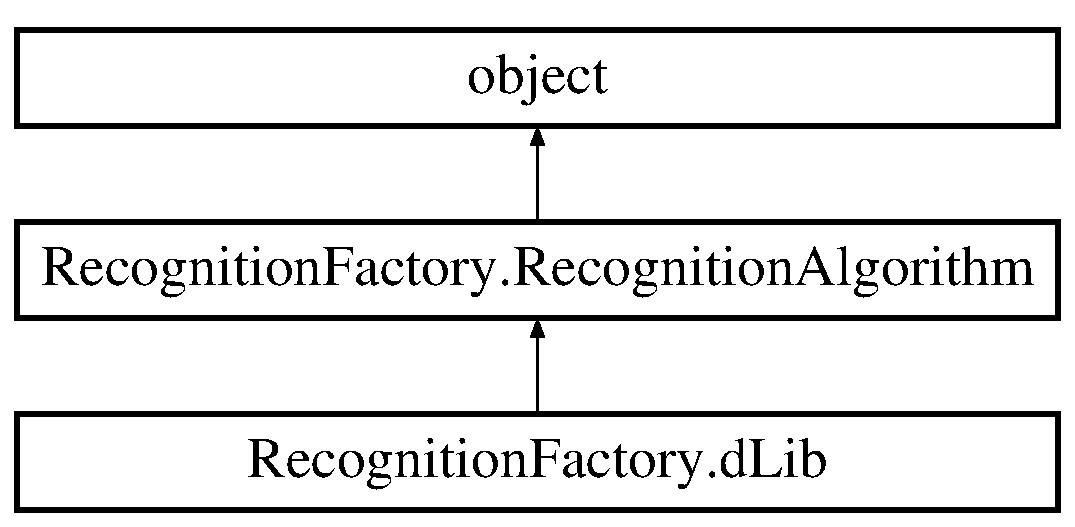
\includegraphics[height=3.000000cm]{classRecognitionFactory_1_1dLib}
\end{center}
\end{figure}
\subsection*{Public Member Functions}
\begin{DoxyCompactItemize}
\item 
def \hyperlink{classRecognitionFactory_1_1dLib_a7bb73498790a1728080d244b168708da}{\-\_\-\-\_\-init\-\_\-\-\_\-}
\begin{DoxyCompactList}\small\item\em Initialization Function. \end{DoxyCompactList}\item 
def \hyperlink{classRecognitionFactory_1_1dLib_acc97bda5d45cea6211c579800157cfff}{calc\-\_\-face\-\_\-descriptor}
\begin{DoxyCompactList}\small\item\em Calculates the face descriptor according to the bounding box and the image given. \end{DoxyCompactList}\item 
def \hyperlink{classRecognitionFactory_1_1dLib_a40973a6daa92cf8801b0e3651a29c83c}{calc\-\_\-face\-\_\-descriptor\-\_\-aligned\-Image}
\begin{DoxyCompactList}\small\item\em Calculates the face descriptor according to an already aligned face. \end{DoxyCompactList}\item 
def \hyperlink{classRecognitionFactory_1_1dLib_adf0aa845ca2d8ff90bb685722dc77f2d}{compare}
\begin{DoxyCompactList}\small\item\em It compares two face descriptors and it will return the similarity between them. \end{DoxyCompactList}\item 
\hypertarget{classRecognitionFactory_1_1dLib_ad428d6482b785537ae2e86113c6ba17d}{def {\bfseries draw}}\label{classRecognitionFactory_1_1dLib_ad428d6482b785537ae2e86113c6ba17d}

\end{DoxyCompactItemize}
\subsection*{Public Attributes}
\begin{DoxyCompactItemize}
\item 
\hypertarget{classRecognitionFactory_1_1dLib_a6957e65ac5c057c4df83936944e779b5}{{\bfseries facerec}}\label{classRecognitionFactory_1_1dLib_a6957e65ac5c057c4df83936944e779b5}

\item 
\hypertarget{classRecognitionFactory_1_1dLib_a0ac95514f25342efc41b1525381e1722}{{\bfseries sp}}\label{classRecognitionFactory_1_1dLib_a0ac95514f25342efc41b1525381e1722}

\item 
\hypertarget{classRecognitionFactory_1_1dLib_a02d8bf3bba4ddfde4d823a5bb3973c27}{{\bfseries path\-\_\-to\-\_\-vectors}}\label{classRecognitionFactory_1_1dLib_a02d8bf3bba4ddfde4d823a5bb3973c27}

\item 
\hypertarget{classRecognitionFactory_1_1dLib_aa3414f96351806052f4343677c34c4da}{{\bfseries threshold}}\label{classRecognitionFactory_1_1dLib_aa3414f96351806052f4343677c34c4da}

\item 
\hypertarget{classRecognitionFactory_1_1dLib_a9505ee9b34f1b5a70390e7fd137b02ee}{{\bfseries aligned\-Face}}\label{classRecognitionFactory_1_1dLib_a9505ee9b34f1b5a70390e7fd137b02ee}

\end{DoxyCompactItemize}
\subsection*{Additional Inherited Members}


\subsection{Constructor \& Destructor Documentation}
\hypertarget{classRecognitionFactory_1_1dLib_a7bb73498790a1728080d244b168708da}{\index{Recognition\-Factory\-::d\-Lib@{Recognition\-Factory\-::d\-Lib}!\-\_\-\-\_\-init\-\_\-\-\_\-@{\-\_\-\-\_\-init\-\_\-\-\_\-}}
\index{\-\_\-\-\_\-init\-\_\-\-\_\-@{\-\_\-\-\_\-init\-\_\-\-\_\-}!RecognitionFactory::dLib@{Recognition\-Factory\-::d\-Lib}}
\subsubsection[{\-\_\-\-\_\-init\-\_\-\-\_\-}]{\setlength{\rightskip}{0pt plus 5cm}def Recognition\-Factory.\-d\-Lib.\-\_\-\-\_\-init\-\_\-\-\_\- (
\begin{DoxyParamCaption}
\item[{}]{self}
\end{DoxyParamCaption}
)}}\label{classRecognitionFactory_1_1dLib_a7bb73498790a1728080d244b168708da}


Initialization Function. 

It will load the models and set the thresholds. 

\subsection{Member Function Documentation}
\hypertarget{classRecognitionFactory_1_1dLib_acc97bda5d45cea6211c579800157cfff}{\index{Recognition\-Factory\-::d\-Lib@{Recognition\-Factory\-::d\-Lib}!calc\-\_\-face\-\_\-descriptor@{calc\-\_\-face\-\_\-descriptor}}
\index{calc\-\_\-face\-\_\-descriptor@{calc\-\_\-face\-\_\-descriptor}!RecognitionFactory::dLib@{Recognition\-Factory\-::d\-Lib}}
\subsubsection[{calc\-\_\-face\-\_\-descriptor}]{\setlength{\rightskip}{0pt plus 5cm}def Recognition\-Factory.\-d\-Lib.\-calc\-\_\-face\-\_\-descriptor (
\begin{DoxyParamCaption}
\item[{}]{self, }
\item[{}]{img, }
\item[{}]{bb, }
\item[{}]{landmarks}
\end{DoxyParamCaption}
)}}\label{classRecognitionFactory_1_1dLib_acc97bda5d45cea6211c579800157cfff}


Calculates the face descriptor according to the bounding box and the image given. 


\begin{DoxyParams}{Parameters}
{\em self} & The object \\
\hline
{\em img} & The image acquired by the camera \\
\hline
{\em bb} & The bounding box of the face detected on the image \\
\hline
{\em landmarks} & The 68 landmarks produced by the function align.\-find\-Landmarks(img, bb)\\
\hline
\end{DoxyParams}
\begin{DoxyReturn}{Returns}
The face descriptor (Array of 128\-D). 
\end{DoxyReturn}
\hypertarget{classRecognitionFactory_1_1dLib_a40973a6daa92cf8801b0e3651a29c83c}{\index{Recognition\-Factory\-::d\-Lib@{Recognition\-Factory\-::d\-Lib}!calc\-\_\-face\-\_\-descriptor\-\_\-aligned\-Image@{calc\-\_\-face\-\_\-descriptor\-\_\-aligned\-Image}}
\index{calc\-\_\-face\-\_\-descriptor\-\_\-aligned\-Image@{calc\-\_\-face\-\_\-descriptor\-\_\-aligned\-Image}!RecognitionFactory::dLib@{Recognition\-Factory\-::d\-Lib}}
\subsubsection[{calc\-\_\-face\-\_\-descriptor\-\_\-aligned\-Image}]{\setlength{\rightskip}{0pt plus 5cm}def Recognition\-Factory.\-d\-Lib.\-calc\-\_\-face\-\_\-descriptor\-\_\-aligned\-Image (
\begin{DoxyParamCaption}
\item[{}]{self, }
\item[{}]{img, }
\item[{}]{bb}
\end{DoxyParamCaption}
)}}\label{classRecognitionFactory_1_1dLib_a40973a6daa92cf8801b0e3651a29c83c}


Calculates the face descriptor according to an already aligned face. 


\begin{DoxyParams}{Parameters}
{\em self} & The object \\
\hline
{\em aligned\-Face} & The aligned face \\
\hline
{\em bb} & The bounding box of the face detected on the image\\
\hline
\end{DoxyParams}
\begin{DoxyReturn}{Returns}
The face descriptor (Array of 128\-D). 
\end{DoxyReturn}
\hypertarget{classRecognitionFactory_1_1dLib_adf0aa845ca2d8ff90bb685722dc77f2d}{\index{Recognition\-Factory\-::d\-Lib@{Recognition\-Factory\-::d\-Lib}!compare@{compare}}
\index{compare@{compare}!RecognitionFactory::dLib@{Recognition\-Factory\-::d\-Lib}}
\subsubsection[{compare}]{\setlength{\rightskip}{0pt plus 5cm}def Recognition\-Factory.\-d\-Lib.\-compare (
\begin{DoxyParamCaption}
\item[{}]{self, }
\item[{}]{face\-\_\-descriptor1, }
\item[{}]{face\-\_\-descriptor2}
\end{DoxyParamCaption}
)}}\label{classRecognitionFactory_1_1dLib_adf0aa845ca2d8ff90bb685722dc77f2d}


It compares two face descriptors and it will return the similarity between them. 


\begin{DoxyParams}{Parameters}
{\em rep1} & First face descriptor \\
\hline
{\em rep2} & Second face descriptor\\
\hline
\end{DoxyParams}
\begin{DoxyReturn}{Returns}
Similairty value 
\end{DoxyReturn}


The documentation for this class was generated from the following file\-:\begin{DoxyCompactItemize}
\item 
py/Recognition\-Factory.\-py\end{DoxyCompactItemize}

\hypertarget{classRecognitionFactory_1_1OpenFace}{}\section{Recognition\+Factory.\+Open\+Face Class Reference}
\label{classRecognitionFactory_1_1OpenFace}\index{Recognition\+Factory.\+Open\+Face@{Recognition\+Factory.\+Open\+Face}}
Inheritance diagram for Recognition\+Factory.\+Open\+Face\+:\begin{figure}[H]
\begin{center}
\leavevmode
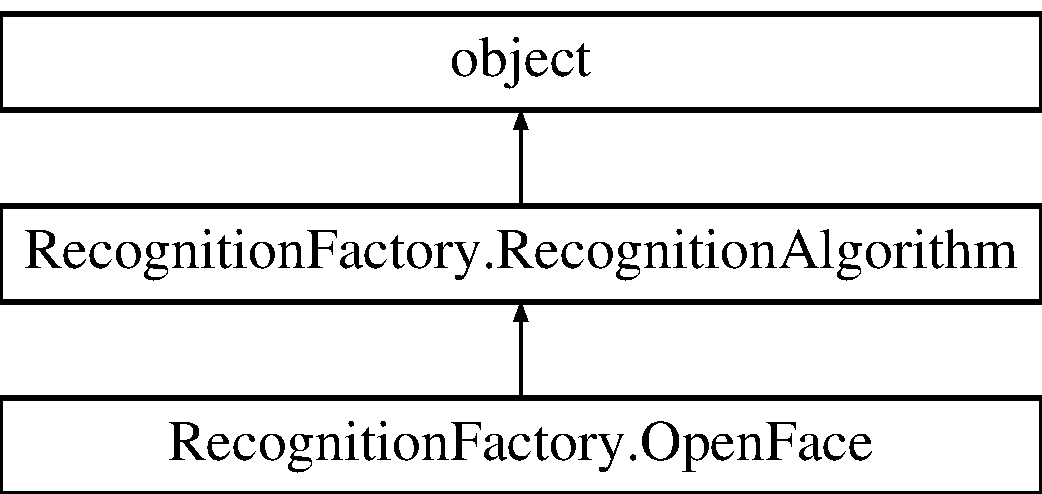
\includegraphics[height=3.000000cm]{classRecognitionFactory_1_1OpenFace}
\end{center}
\end{figure}
\subsection*{Public Member Functions}
\begin{DoxyCompactItemize}
\item 
def {\bfseries \+\_\+\+\_\+init\+\_\+\+\_\+} (self)\hypertarget{classRecognitionFactory_1_1OpenFace_a555a6f98154c13480cd0221bbb616cdc}{}\label{classRecognitionFactory_1_1OpenFace_a555a6f98154c13480cd0221bbb616cdc}

\item 
def \hyperlink{classRecognitionFactory_1_1OpenFace_a836912f1319b9a6b433439514b411e85}{calc\+\_\+face\+\_\+descriptor} (self, img, bb, landmarks)
\begin{DoxyCompactList}\small\item\em According to the image given, it will align the face, apply the preprocessing technique (if aplicable) and then forward through the neural network. \end{DoxyCompactList}\item 
def \hyperlink{classRecognitionFactory_1_1OpenFace_aaf88498d63d98982547f19ee314e5bba}{calc\+\_\+face\+\_\+descriptor\+\_\+aligned\+Image} (self, aligned\+Face, bb)
\begin{DoxyCompactList}\small\item\em According to the face image given, it will apply the preprocessing technique (if aplicable) and then forward through the neural network. \end{DoxyCompactList}\item 
def \hyperlink{classRecognitionFactory_1_1OpenFace_afa0790d2f75b5191265048c584dbb858}{compare} (self, rep1, rep2)
\begin{DoxyCompactList}\small\item\em Given two face descriptors it subtract one to the other and then calculates the norm of the vector. \end{DoxyCompactList}\end{DoxyCompactItemize}
\subsection*{Public Attributes}
\begin{DoxyCompactItemize}
\item 
{\bfseries align}\hypertarget{classRecognitionFactory_1_1OpenFace_a1c901bdf709de3d7e1b40093af926974}{}\label{classRecognitionFactory_1_1OpenFace_a1c901bdf709de3d7e1b40093af926974}

\item 
{\bfseries openface\+Model\+Dir}\hypertarget{classRecognitionFactory_1_1OpenFace_a1ee73330a23fce8a6ca41231d778ec91}{}\label{classRecognitionFactory_1_1OpenFace_a1ee73330a23fce8a6ca41231d778ec91}

\item 
{\bfseries path\+\_\+to\+\_\+descriptors}\hypertarget{classRecognitionFactory_1_1OpenFace_acaa350f52e5e1a71b2d6643403ec1af1}{}\label{classRecognitionFactory_1_1OpenFace_acaa350f52e5e1a71b2d6643403ec1af1}

\item 
{\bfseries net}\hypertarget{classRecognitionFactory_1_1OpenFace_a4cd893ba8a2c3882481901c1093c3ae3}{}\label{classRecognitionFactory_1_1OpenFace_a4cd893ba8a2c3882481901c1093c3ae3}

\item 
{\bfseries threshold}\hypertarget{classRecognitionFactory_1_1OpenFace_a334cc50444b6906a8c08ec658c8f5438}{}\label{classRecognitionFactory_1_1OpenFace_a334cc50444b6906a8c08ec658c8f5438}

\item 
{\bfseries aligned\+Face}\hypertarget{classRecognitionFactory_1_1OpenFace_a1acaa386b19695644e18eab416f390ee}{}\label{classRecognitionFactory_1_1OpenFace_a1acaa386b19695644e18eab416f390ee}

\end{DoxyCompactItemize}
\subsection*{Additional Inherited Members}


\subsection{Member Function Documentation}
\index{Recognition\+Factory\+::\+Open\+Face@{Recognition\+Factory\+::\+Open\+Face}!calc\+\_\+face\+\_\+descriptor@{calc\+\_\+face\+\_\+descriptor}}
\index{calc\+\_\+face\+\_\+descriptor@{calc\+\_\+face\+\_\+descriptor}!Recognition\+Factory\+::\+Open\+Face@{Recognition\+Factory\+::\+Open\+Face}}
\subsubsection[{\texorpdfstring{calc\+\_\+face\+\_\+descriptor(self, img, bb, landmarks)}{calc_face_descriptor(self, img, bb, landmarks)}}]{\setlength{\rightskip}{0pt plus 5cm}def Recognition\+Factory.\+Open\+Face.\+calc\+\_\+face\+\_\+descriptor (
\begin{DoxyParamCaption}
\item[{}]{self, }
\item[{}]{img, }
\item[{}]{bb, }
\item[{}]{landmarks}
\end{DoxyParamCaption}
)}\hypertarget{classRecognitionFactory_1_1OpenFace_a836912f1319b9a6b433439514b411e85}{}\label{classRecognitionFactory_1_1OpenFace_a836912f1319b9a6b433439514b411e85}


According to the image given, it will align the face, apply the preprocessing technique (if aplicable) and then forward through the neural network. 


\begin{DoxyParams}{Parameters}
{\em img} & Image acquired by the camera \\
\hline
{\em bb} & Bounding box that delineates the biggest face found on the image\\
\hline
\end{DoxyParams}

\begin{DoxyRetVals}{Return values}
{\em The} & face descriptor \\
\hline
\end{DoxyRetVals}
\index{Recognition\+Factory\+::\+Open\+Face@{Recognition\+Factory\+::\+Open\+Face}!calc\+\_\+face\+\_\+descriptor\+\_\+aligned\+Image@{calc\+\_\+face\+\_\+descriptor\+\_\+aligned\+Image}}
\index{calc\+\_\+face\+\_\+descriptor\+\_\+aligned\+Image@{calc\+\_\+face\+\_\+descriptor\+\_\+aligned\+Image}!Recognition\+Factory\+::\+Open\+Face@{Recognition\+Factory\+::\+Open\+Face}}
\subsubsection[{\texorpdfstring{calc\+\_\+face\+\_\+descriptor\+\_\+aligned\+Image(self, aligned\+Face, bb)}{calc_face_descriptor_alignedImage(self, alignedFace, bb)}}]{\setlength{\rightskip}{0pt plus 5cm}def Recognition\+Factory.\+Open\+Face.\+calc\+\_\+face\+\_\+descriptor\+\_\+aligned\+Image (
\begin{DoxyParamCaption}
\item[{}]{self, }
\item[{}]{aligned\+Face, }
\item[{}]{bb}
\end{DoxyParamCaption}
)}\hypertarget{classRecognitionFactory_1_1OpenFace_aaf88498d63d98982547f19ee314e5bba}{}\label{classRecognitionFactory_1_1OpenFace_aaf88498d63d98982547f19ee314e5bba}


According to the face image given, it will apply the preprocessing technique (if aplicable) and then forward through the neural network. 


\begin{DoxyParams}{Parameters}
{\em img} & Face image gave by the face detector \\
\hline
{\em bb} & Not used, can be anything\\
\hline
\end{DoxyParams}

\begin{DoxyRetVals}{Return values}
{\em The} & face descriptor \\
\hline
\end{DoxyRetVals}
\index{Recognition\+Factory\+::\+Open\+Face@{Recognition\+Factory\+::\+Open\+Face}!compare@{compare}}
\index{compare@{compare}!Recognition\+Factory\+::\+Open\+Face@{Recognition\+Factory\+::\+Open\+Face}}
\subsubsection[{\texorpdfstring{compare(self, rep1, rep2)}{compare(self, rep1, rep2)}}]{\setlength{\rightskip}{0pt plus 5cm}def Recognition\+Factory.\+Open\+Face.\+compare (
\begin{DoxyParamCaption}
\item[{}]{self, }
\item[{}]{rep1, }
\item[{}]{rep2}
\end{DoxyParamCaption}
)}\hypertarget{classRecognitionFactory_1_1OpenFace_afa0790d2f75b5191265048c584dbb858}{}\label{classRecognitionFactory_1_1OpenFace_afa0790d2f75b5191265048c584dbb858}


Given two face descriptors it subtract one to the other and then calculates the norm of the vector. 

This is also called the similarity between two vectors. It is usally made on the face verification process and facetracking. The higher the value the more likely that it is a different person.


\begin{DoxyParams}{Parameters}
{\em face\+\_\+descriptor1} & Face image gave by the face detector \\
\hline
{\em face\+\_\+descriptor2} & Bounding box that delineates the biggest face found on the image (in this case is the face image dimensions)\\
\hline
\end{DoxyParams}

\begin{DoxyRetVals}{Return values}
{\em Value} & of similarity between vectors \\
\hline
\end{DoxyRetVals}


The documentation for this class was generated from the following file\+:\begin{DoxyCompactItemize}
\item 
py/Recognition\+Factory.\+py\end{DoxyCompactItemize}

\hypertarget{classRecognitionFactory_1_1RecognitionAlgorithm}{\section{Recognition\-Factory.\-Recognition\-Algorithm Class Reference}
\label{classRecognitionFactory_1_1RecognitionAlgorithm}\index{Recognition\-Factory.\-Recognition\-Algorithm@{Recognition\-Factory.\-Recognition\-Algorithm}}
}


Recognition factory to choose which algorithm will be used.  


Inheritance diagram for Recognition\-Factory.\-Recognition\-Algorithm\-:\begin{figure}[H]
\begin{center}
\leavevmode
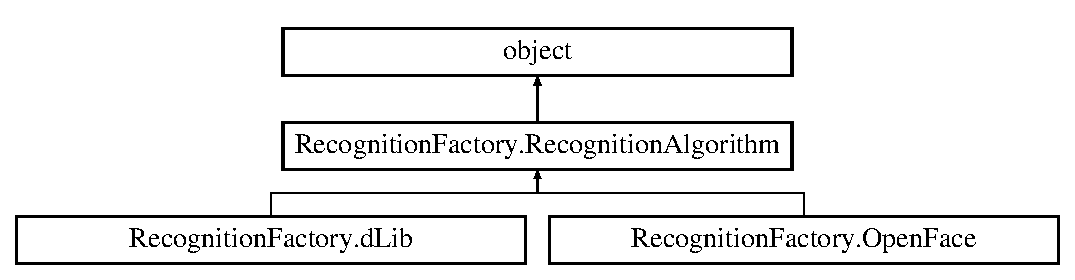
\includegraphics[height=3.000000cm]{classRecognitionFactory_1_1RecognitionAlgorithm}
\end{center}
\end{figure}
\subsection*{Public Member Functions}
\begin{DoxyCompactItemize}
\item 
\hypertarget{classRecognitionFactory_1_1RecognitionAlgorithm_acc15c6c8c13e74e4fa5848141b3a98bb}{def {\bfseries factory}}\label{classRecognitionFactory_1_1RecognitionAlgorithm_acc15c6c8c13e74e4fa5848141b3a98bb}

\end{DoxyCompactItemize}
\subsection*{Static Public Attributes}
\begin{DoxyCompactItemize}
\item 
\hypertarget{classRecognitionFactory_1_1RecognitionAlgorithm_a9d948cf769252cf8bdc07639332203d3}{tuple {\bfseries factory} = staticmethod(factory)}\label{classRecognitionFactory_1_1RecognitionAlgorithm_a9d948cf769252cf8bdc07639332203d3}

\end{DoxyCompactItemize}


\subsection{Detailed Description}
Recognition factory to choose which algorithm will be used. 

(\hyperlink{classRecognitionFactory_1_1dLib}{d\-Lib} or \hyperlink{classRecognitionFactory_1_1OpenFace}{Open\-Face}). 

The documentation for this class was generated from the following file\-:\begin{DoxyCompactItemize}
\item 
py/Recognition\-Factory.\-py\end{DoxyCompactItemize}

%--- End generated contents ---

% Index
\newpage
\phantomsection
\addcontentsline{toc}{chapter}{Index}
\printindex

\end{document}
